\documentclass[letterpaper, 10 pt, conference]{ieeeconf}  % Comment this line out if you need a4paper

%\documentclass[a4paper, 10pt, conference]{ieeeconf}      % Use this line for a4 paper

\IEEEoverridecommandlockouts                              % This command is only needed if 
                                                          % you want to use the \thanks command

\overrideIEEEmargins                                      % Needed to meet printer requirements.

% The following packages can be found on http:\\www.ctan.org
\usepackage{graphics} % for pdf, bitmapped graphics files
\usepackage[dvipdfmx]{graphicx}
\usepackage[dvipdfmx]{color}
\usepackage{epsfig} % for postscript graphics files
\usepackage{mathptmx} % assumes new font selection scheme installed
\usepackage{times} % assumes new font selection scheme installed
\usepackage{amsmath} % assumes amsmath package installed
\usepackage{amssymb}  % assumes amsmath package installed
\usepackage{multicol}
\usepackage{multirow}
\usepackage{url}
\usepackage{caption}
\usepackage[ruled,vlined]{algorithm2e}
%\include{pythonlisting}
\usepackage{algpseudocode}
\usepackage[dvipsnames]{xcolor}
\usepackage{cite}

\setlength\textfloatsep{5pt}

\title{\LARGE \bf
VCO Comparator: An Adaptive Noise Scaling Comparator for High-Precision and Low-Power SAR ADCs
}

\author{Kentaro Yoshioka% <-this % stops a space
%\thanks{*This work was not supported by any organization}% <-this % stops a space
\thanks{
        {\tt\small yoshioka@elec.keio.ac.jp}}
}

\begin{document}

\maketitle
\thispagestyle{empty}
\pagestyle{empty}

%%%%%%%%%%%%%%%%%%%%%%%%%%%%%%%%%%%%%%%%%%%%%%%%%%%%%%%%%%%%%%%%%%%%%%%%%%%%%%%%
\begin{abstract}


\end{abstract}

%%%%%%%%%%%%%%%%%%%%%%%%%%%%%%%%%%%%%%%%%%%%%%%%%%%%%%%%%%%%%%%%%%%%%%%%%%%%%%%%
\section{Introduction}
IoT技術の進展によって身の回りのセンサ数は増え続けている。特に環境情報をセンシングするにはセンサは電池駆動であるため高精度かつ低電力なADCが必要となる。ここ数年でオペアンプを必要としないsuccessive-apporximation-registor ADC (SAR ADC)の低電力化が大きく進み、多くの低電力SAR ADCが提案された\cite{van201010,shikata20120,yoshioka201010,yoshioka20148,zhu201010,tai201411}。一方でこれらの低電力SAR ADCの多くはSNDR<60dBである。This is because realizing high-resolution capacitor digital-to-analog converter (C-DAC) and comparator with small power dissipation is very challenging. 

However, recent trends show resolution extension in low-power SAR ADCs. C-DACはミスマッチ要求を満足するために設計。そのためkT/Cノイズよりも遥かに大きい単位容量を使用し設計されてきた。大きいC-DACはチャージ電力も大きいだけではなく、ADC駆動アンプやレファンレンス生成器の消費電力も増加してしまう。いっぽうで近年の研究は capacitor matching requirements can be significantly relaxed by fully-digital background calibrations \cite{liu201012b,liu201112,mcneill2011all,mcneill2005split} and thus, unit capacitors can be shrunk until kT/C limitations. This greatly reduces the C-DAC power consumption. 
On the other hand, lowering the comparator noise is more challenging. Since the comparator is the only pure-analog component in SAR ADCs, designers must face tradeoffs of noise, power consumption, speed, and PVT variation tolerance.

我々は入力電圧差に応じノイズ性能を適応的に切り替えるVCOベース比較器を提案する\cite{yoshioka201413b}。VCOにて電圧情報を時間領域に変換することで位相ドメインで比較を行う。VCO比較器は位相比較器のデッドゾーンを用いることで位相差が十分開くまで発振を続けるeye-opening技術により、入力電圧差に応じた適応的にノイズを低減する。
結果としてVCO比較器はノイズ性能に応じて消費電力もスケールし、高精度SAR ADCにて支配的となってしまう比較器の消費電力を大きくカットする。比較機のメタステーブル状態から2つのノイズモードの切り替えを行うdata-driven-noise-reduction (DDNR)比較器\cite{harpe201310b}と比べ、比較器電力を最大半分に削減する。
また65nm CMOSの13bit SAR ADCでVCO比較器のコンセプトを実証。the ADC achieves SNDR 66 dB at 1 MS/s with FoM of 29fJ/conv.-step. Since the VCO comparator is mainly based on inverters and other simple logic cells, benefits can be granted by process scaling.
著者の知る限りVCO比較器は初めて入力差に適応するノイズ低減を達成し、ref.\cite{yoshioka201413b}発表後から様々な低電力高分解能(12-15bit) SAR ADCにVCO比較器は使用されてきた\cite{ding20190, luo2020input, hsieh20180, li2019design, li202065, almarashli2017nyquist, shim2017edge, zhu201914, pan202012, lee2019fast}。

本論文ではref.\cite{yoshioka201413b}に加え、VCO比較器の動作原理やノイズ特性、詳細回路インプリ、そしてPVTばらつき下におけるノイズ変動耐性について詳細な解析結果を追加した。
本論文の構成は以下である。二章では従来高精度比較器の課題、3章ではVCO比較器の原理と解析、4章では回路インプリについてそして最後に5章で測定結果を示し最後にまとめる。


\section{Conventional low-power high-resolution comparators}
\begin{figure}[ht!]
\centering
 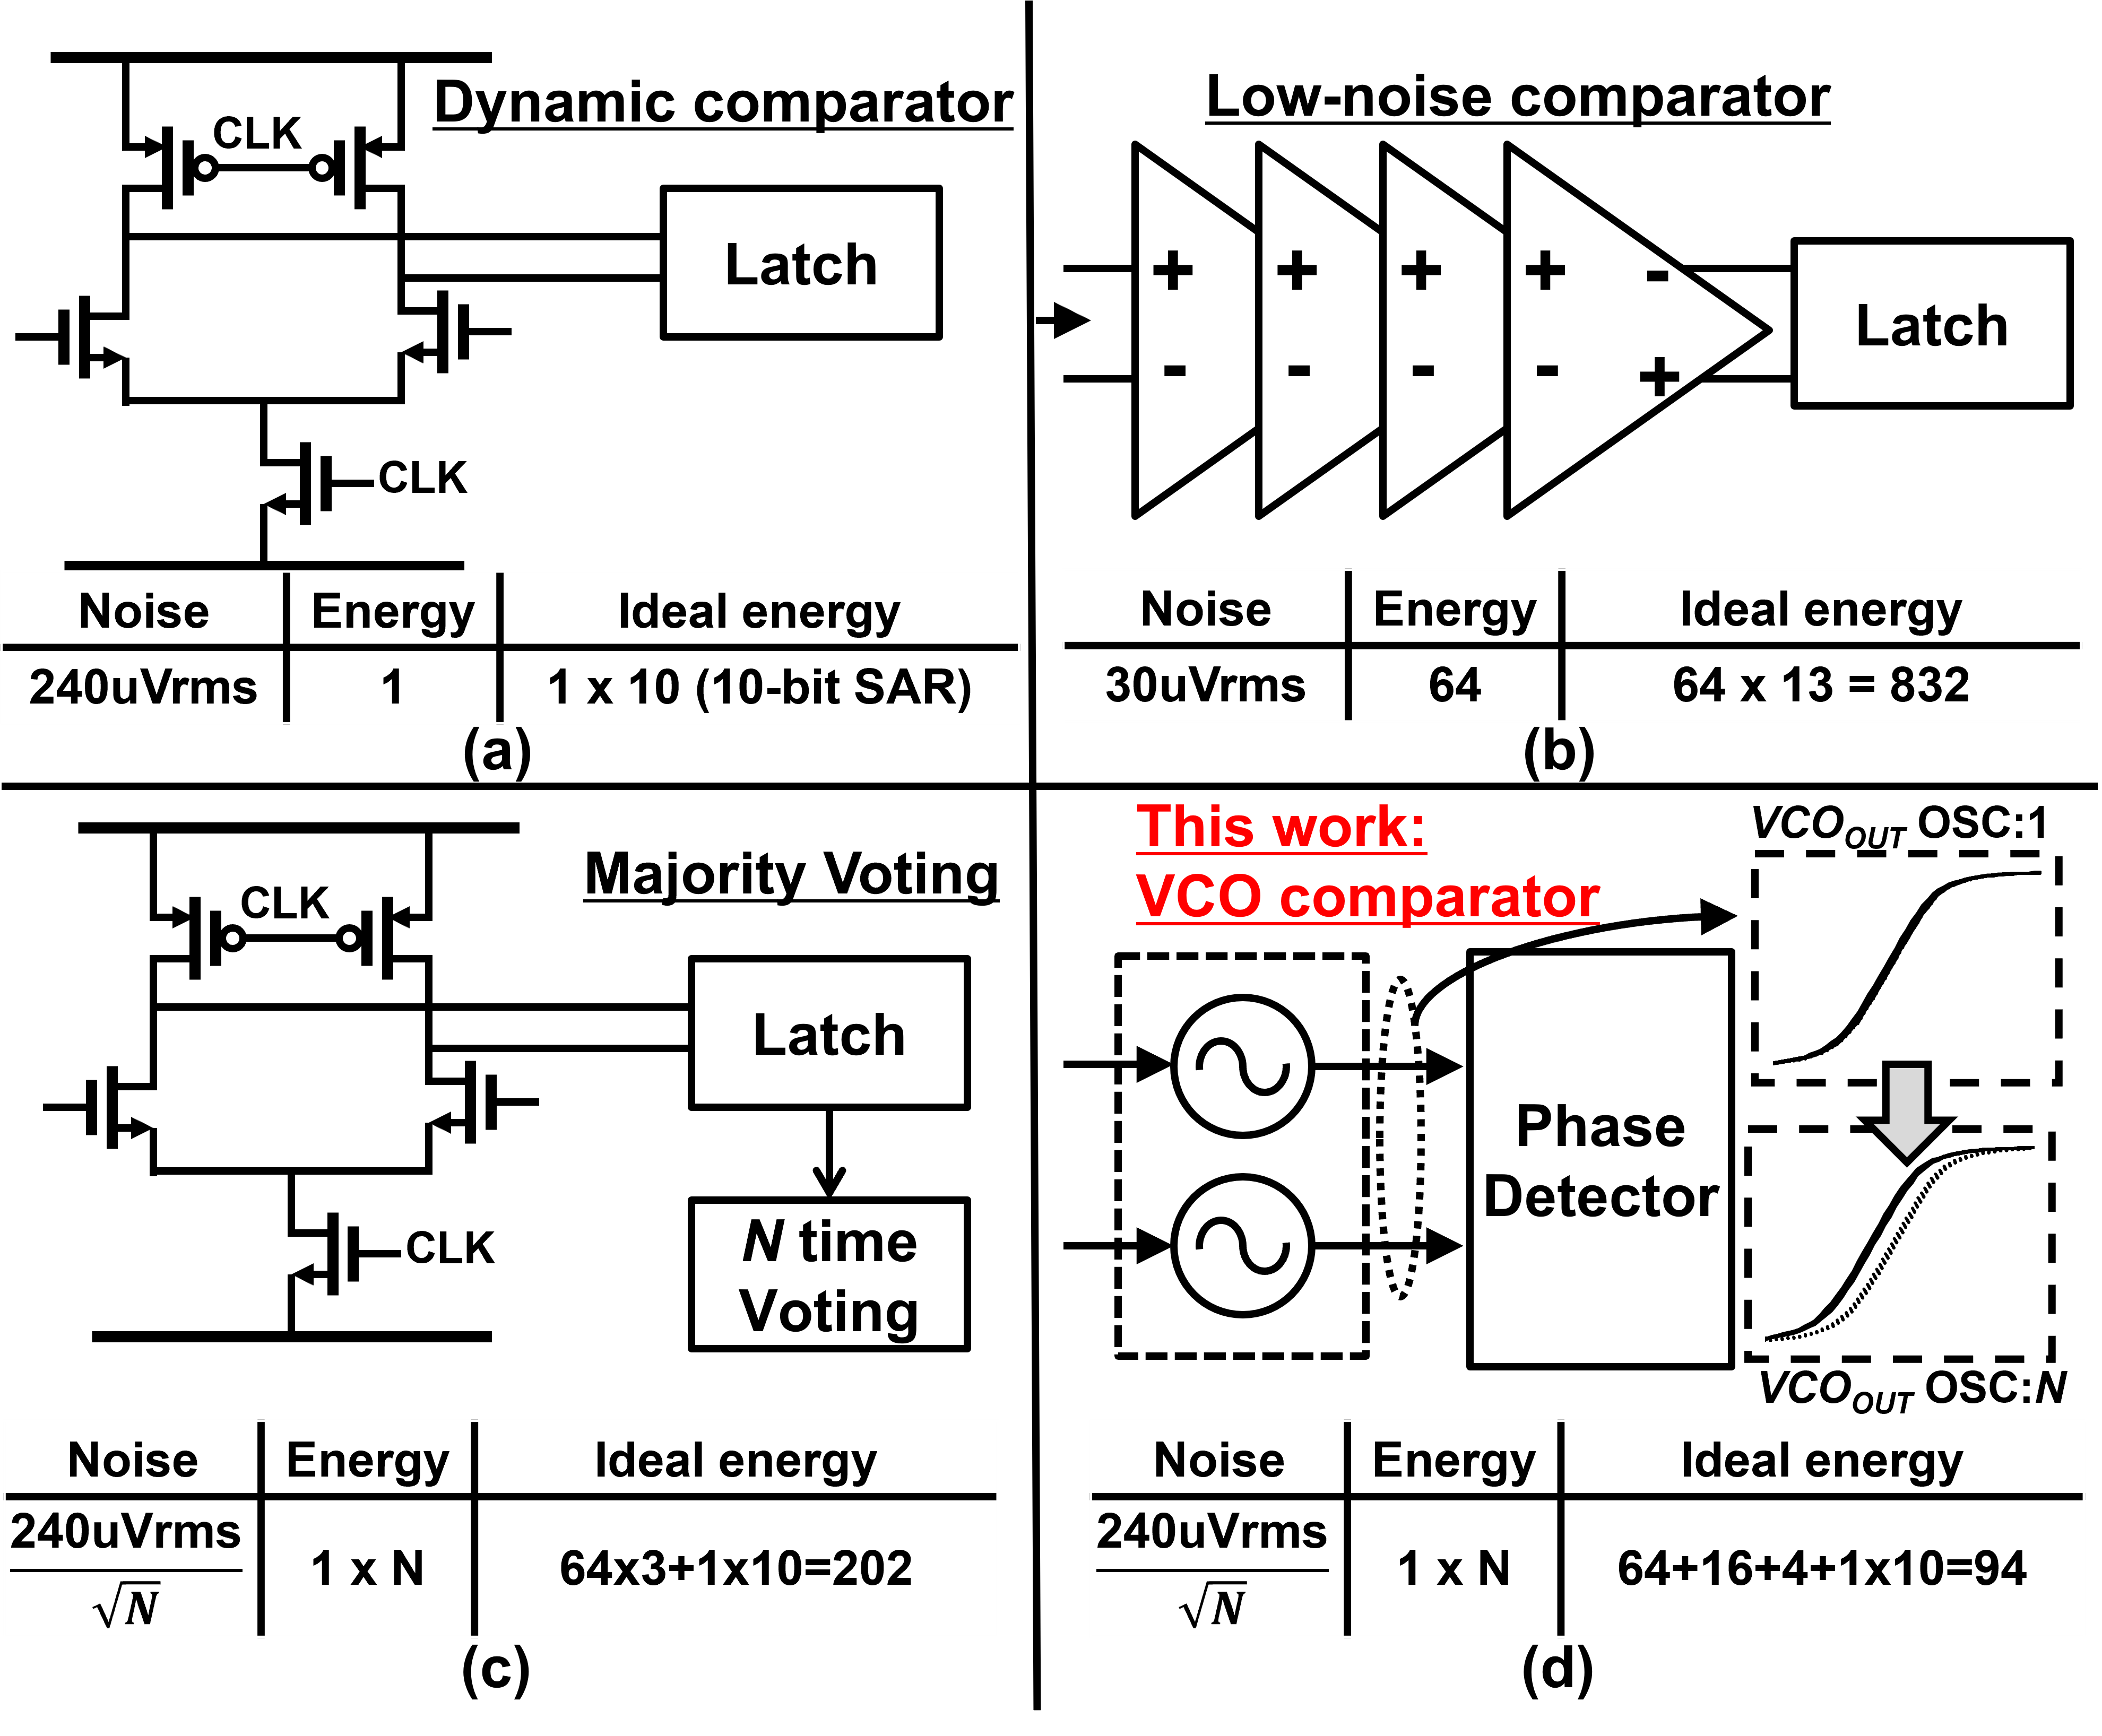
\includegraphics[width=0.5\textwidth]{figs/fig1_r1.png}
  \captionsetup{font=footnotesize}
  \caption{\textbf{ADC}}
  \label{highlight}
\end{figure}
\begin{figure}[ht!]
\centering
 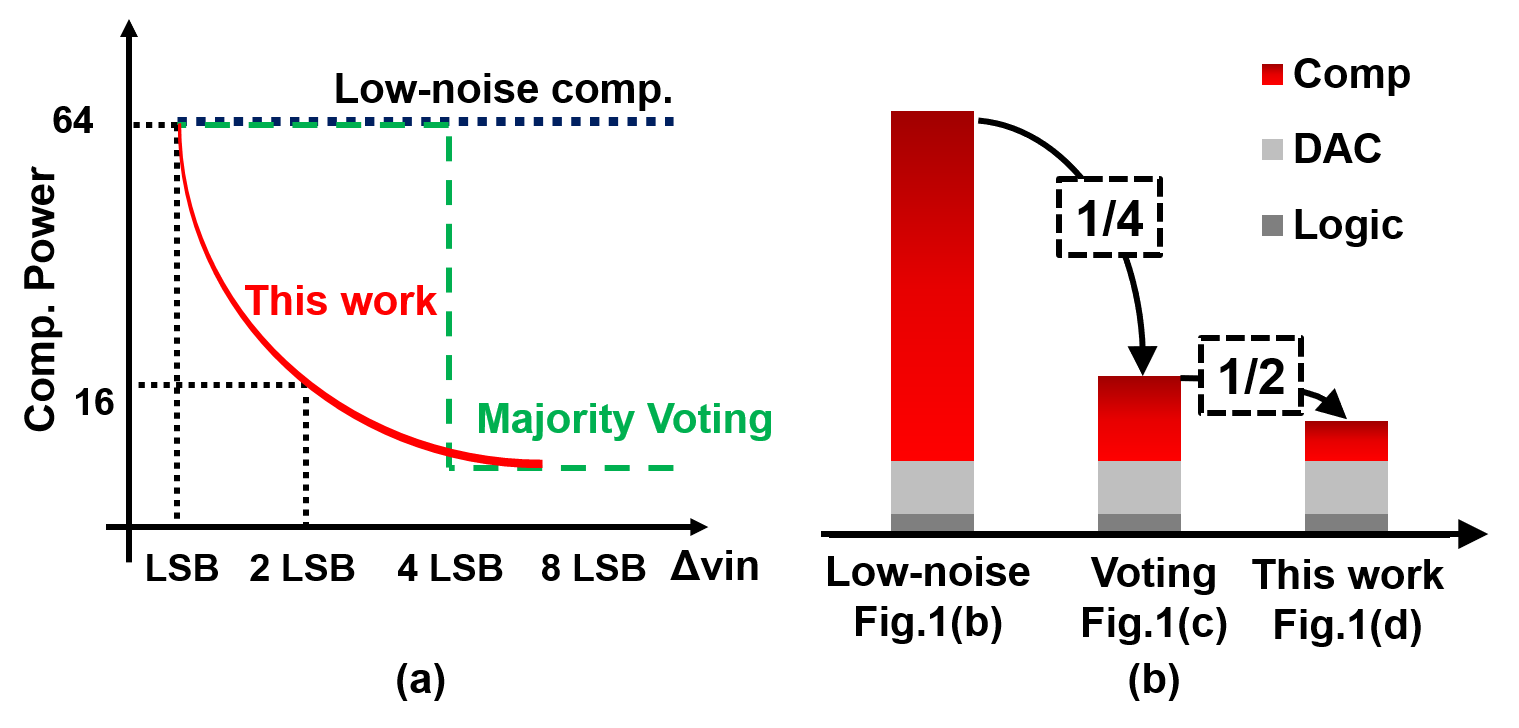
\includegraphics[width=0.4\textwidth]{figs/fig2.png}
  \captionsetup{font=footnotesize}
  \caption{\textbf{ADC}}
  \label{highlight}
\end{figure}
\begin{figure}[ht!]
\centering
 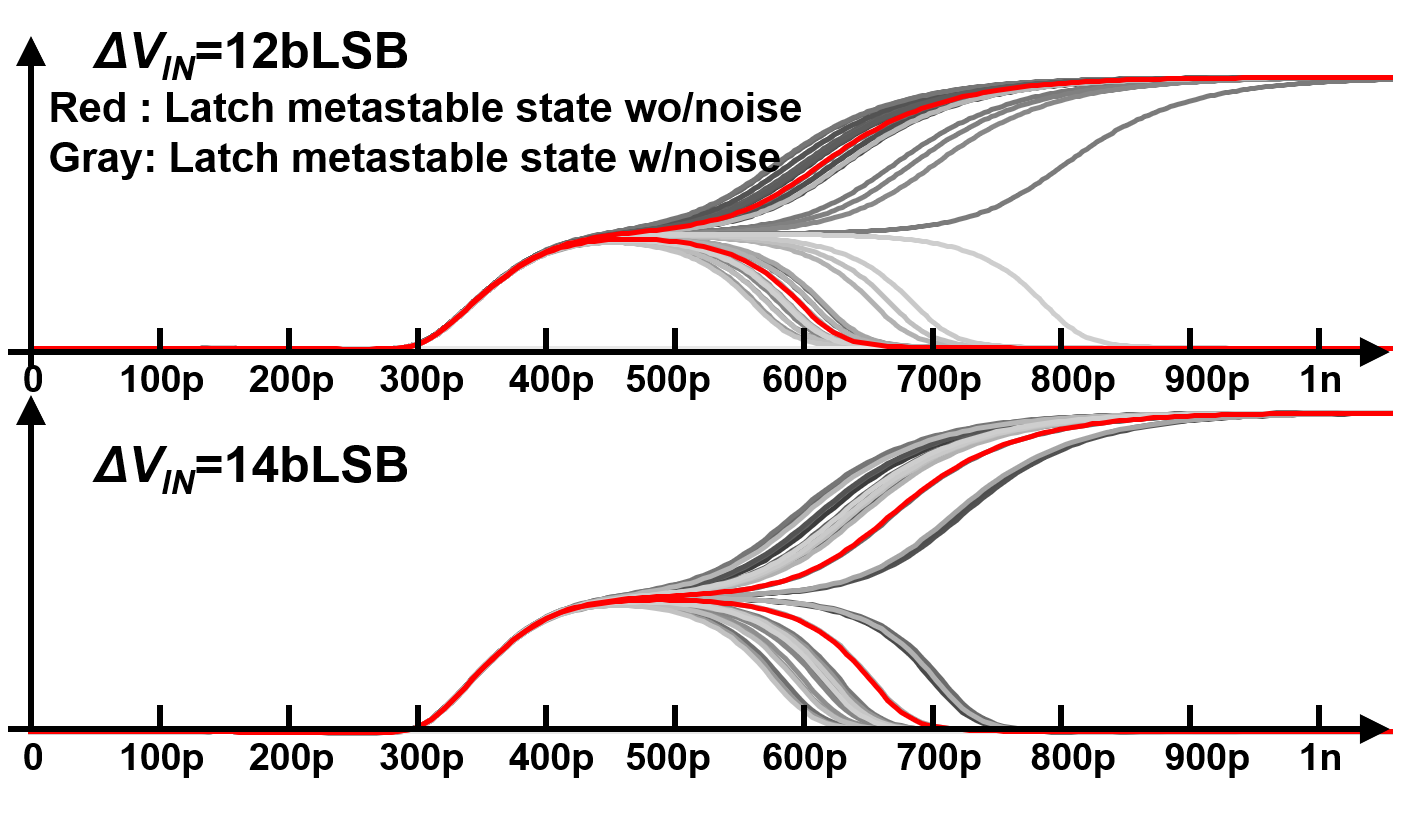
\includegraphics[width=0.4\textwidth]{figs/conventional-strongarm.png}
  \captionsetup{font=footnotesize}
  \caption{\textbf{ADC}}
  \label{highlight}
\end{figure}

Fig.1 (a) shows a typical comparator \cite{miyahara2008low} used in low-power SAR ADCs. Although noise can be reduced by limiting the bandwidth of the preamp stage, a typical design has input referred noise (IRN) of 10b resolution. Fig.1(b) shows a comparator used in 14b SAR ADC \cite{hesener200714b}. The comparator IRN is reduced by increasing the preamp stages before the latch. However, during the successive approximation (SA) conversion, D*vin* differs each cycle(図). Moreover, D*vin* < 1 LSB only occurs once, which is the situation when comparator noise requirement is most strict. In other words, the comparator noise requirement is relaxed at other cycles and using a low-noise comparator for all of the cycles is inefficient. 

To cut down comparator power, ref.\cite{harpe201310b} propose data-driven noise reduction (DDNR) technique, where the comparator triggers majority voting when the D*vin* is sufficiently small from comparator meta-stability \cite{shikata20120}. The comparator output is decided given the result of *N* time voting, and comparator IRN improves as (式)

入力差が小さい時のみに低ノイズな比較を行うため、大きく比較器電力を削減することができる。

Here, we analyze the comparator power of the above techniques. Ideally, to halve the comparator IRN, 4x much power is consumed. Therefore, when the power of 10b resolution comparator is normalized as 1, the power of 13b comparator can be described as:

Then, the total comparator power of 13b SAR ADC will be:(式)

Next, we will assume that DDNR done with 10b comparator. If the D*vin* is smaller than 4xLSB (which corresponds to 11b resolution), majority voting will be done.

The comparator power can reduced by over 1/4.  D*vin* versus comparator power is shown in Fig.2(a), and the power of majority voting comparator is plotted in dashed green line. There is brick wall at D*vin* of 11b resolution, and large power is consumed below that voltage. もしDvinレベルに応じ更に細かく比較機のノイズレベルを切り替えられたら更に比較器電力をへらすことができる。For an example, only 4 LSB level of IRN is required if D*vin* = 4 LSB. 

However, it is challenging for the comparator to detect the value of D*vin* levels(図). The meta-stable time of the typical low-power 10b comparator is determined by preamp noise if the D*vin* is lower than 4 LSB, and therefore, it cannot distinguish the input level (D*vin*) in that range. In addition, comparator meta-stable time drifts heavily by PVT variation and robust operation is difficult.

またTime domain comparators such as delay comparator \cite{agnes20089} はプロセススケーラビリティと低電力動作能力を持ち、発展が期待されている. 一方でこれらのnoise characteristics are not enough for high-resolution ADCs.

\section{Concept of VCO Comparators}
\subsection{VCO Comparator Fundamentals}
\begin{figure*}[ht!]
\centering
 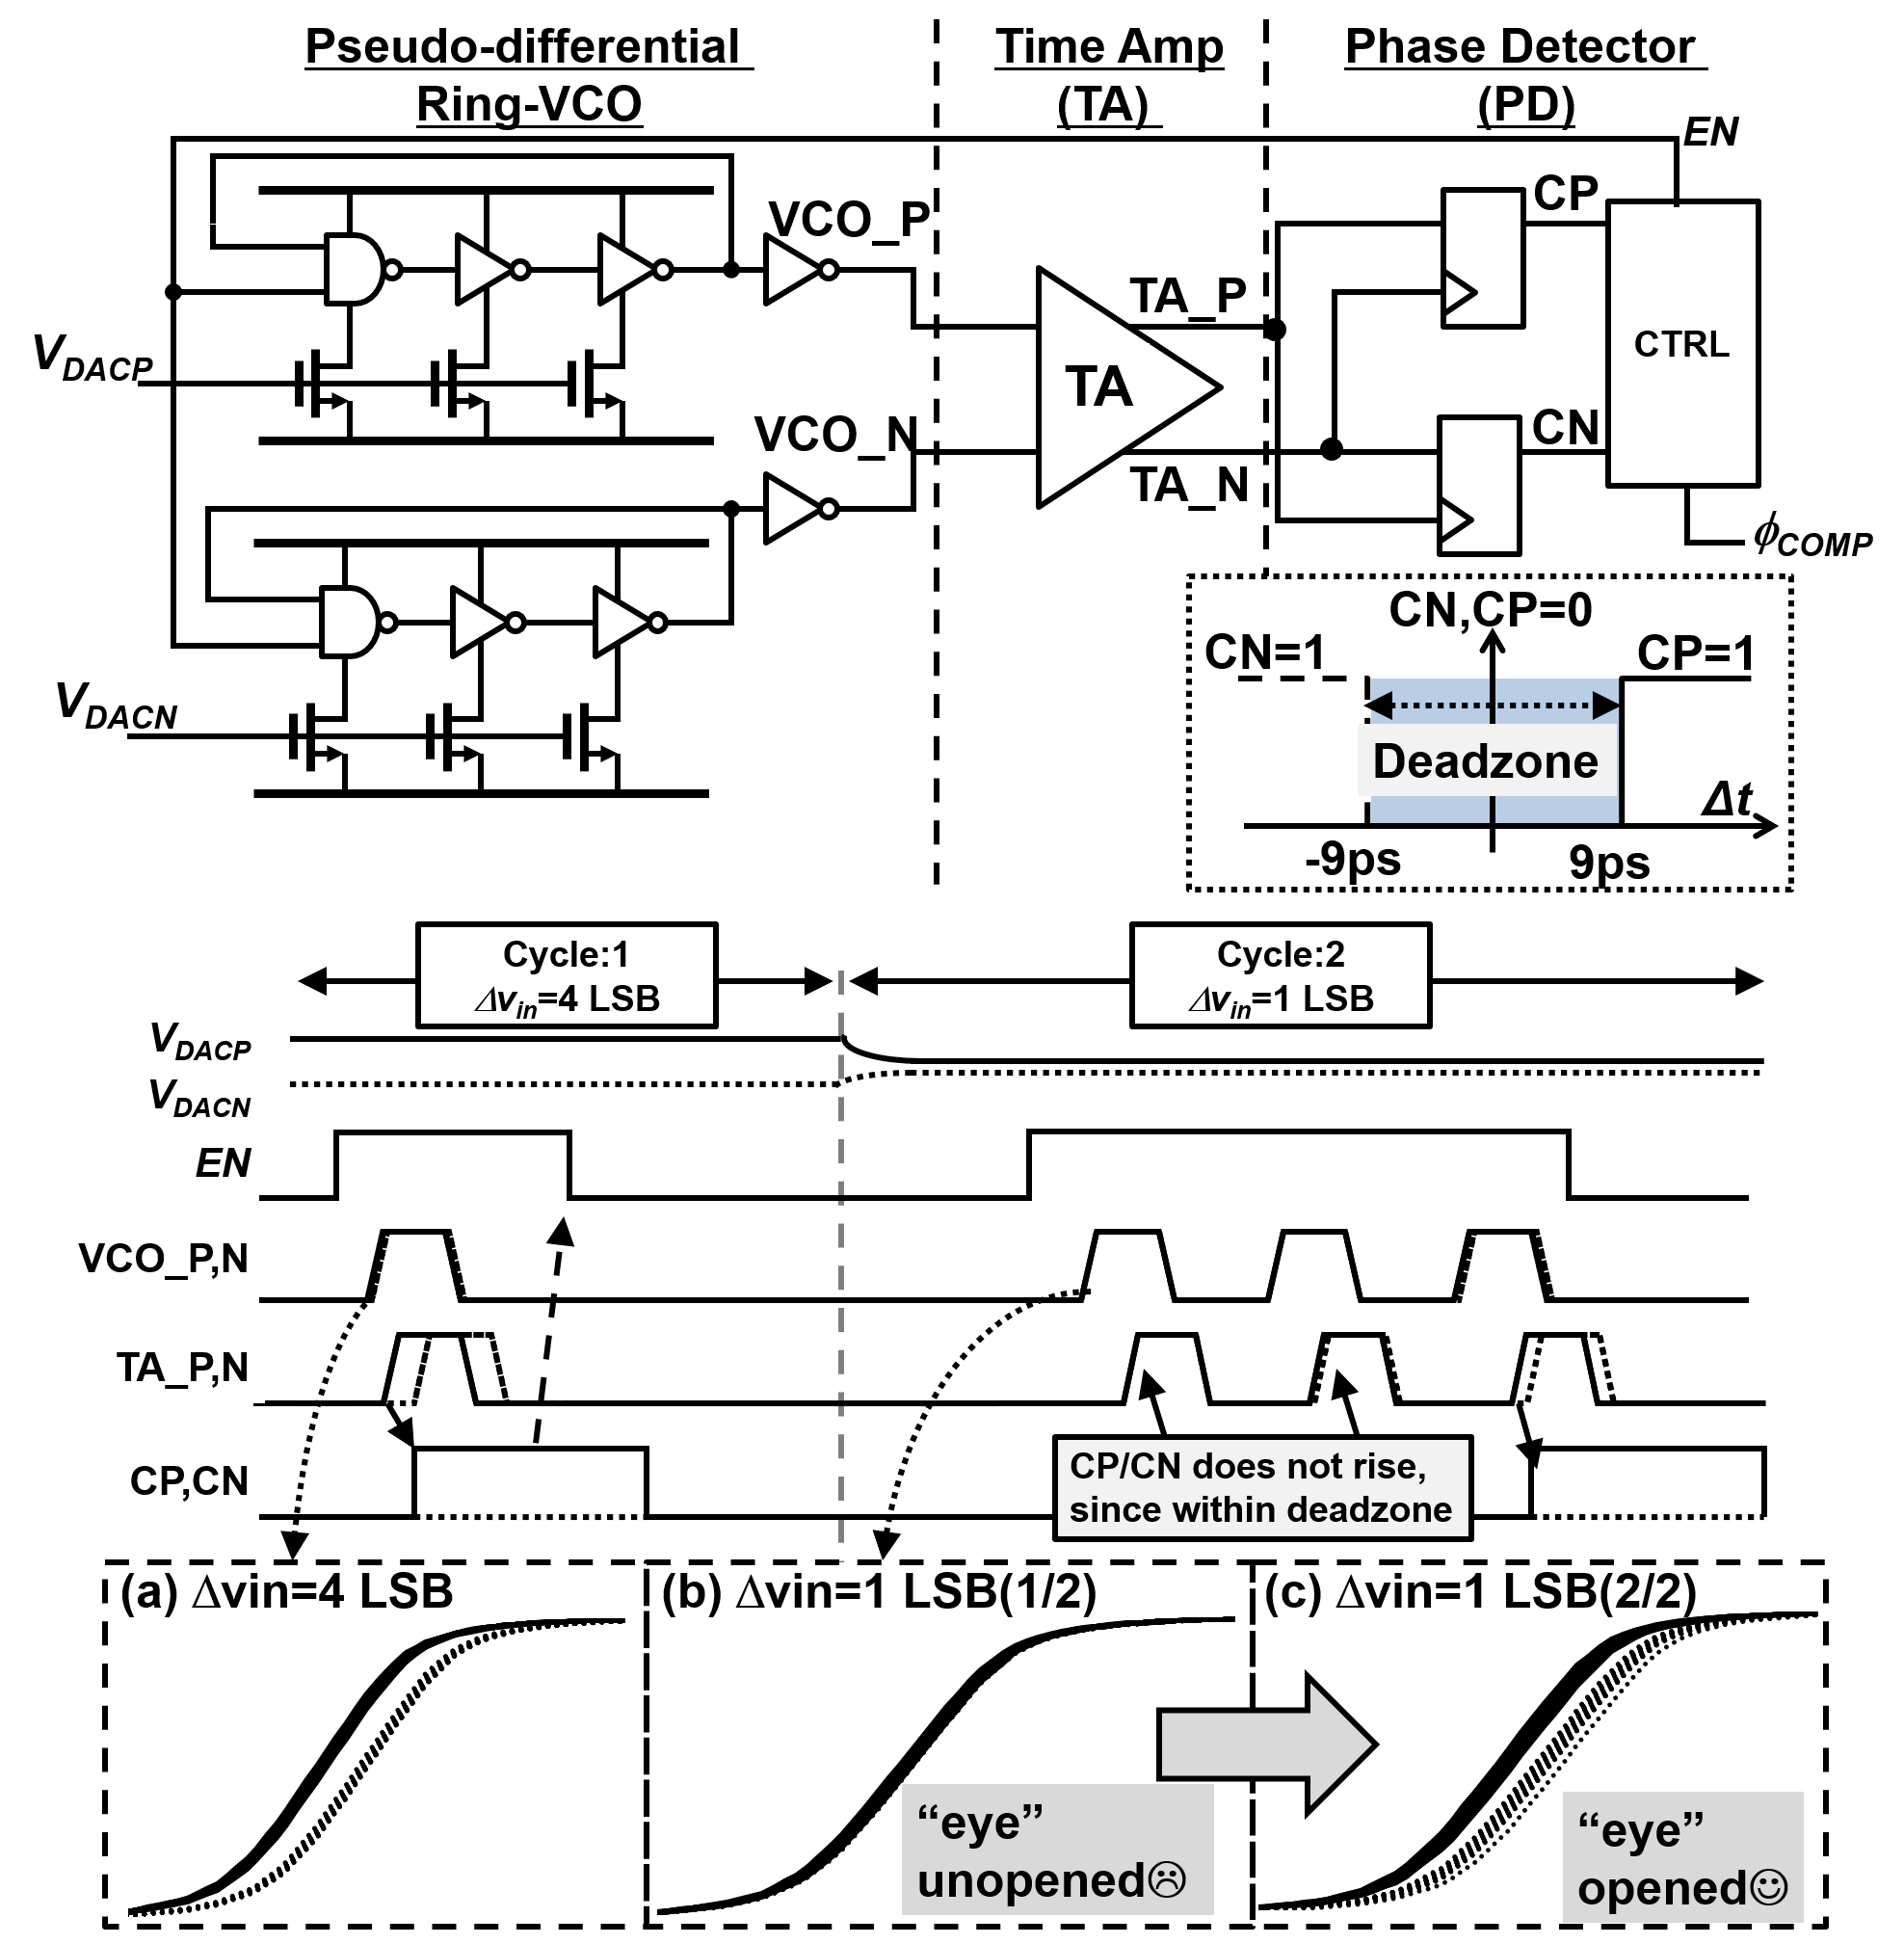
\includegraphics[width=0.9\textwidth]{figs/full.png}
  \captionsetup{font=footnotesize}
  \caption{\textbf{ADC}}
  \label{highlight}
\end{figure*}

\begin{figure}[ht!]
\centering
 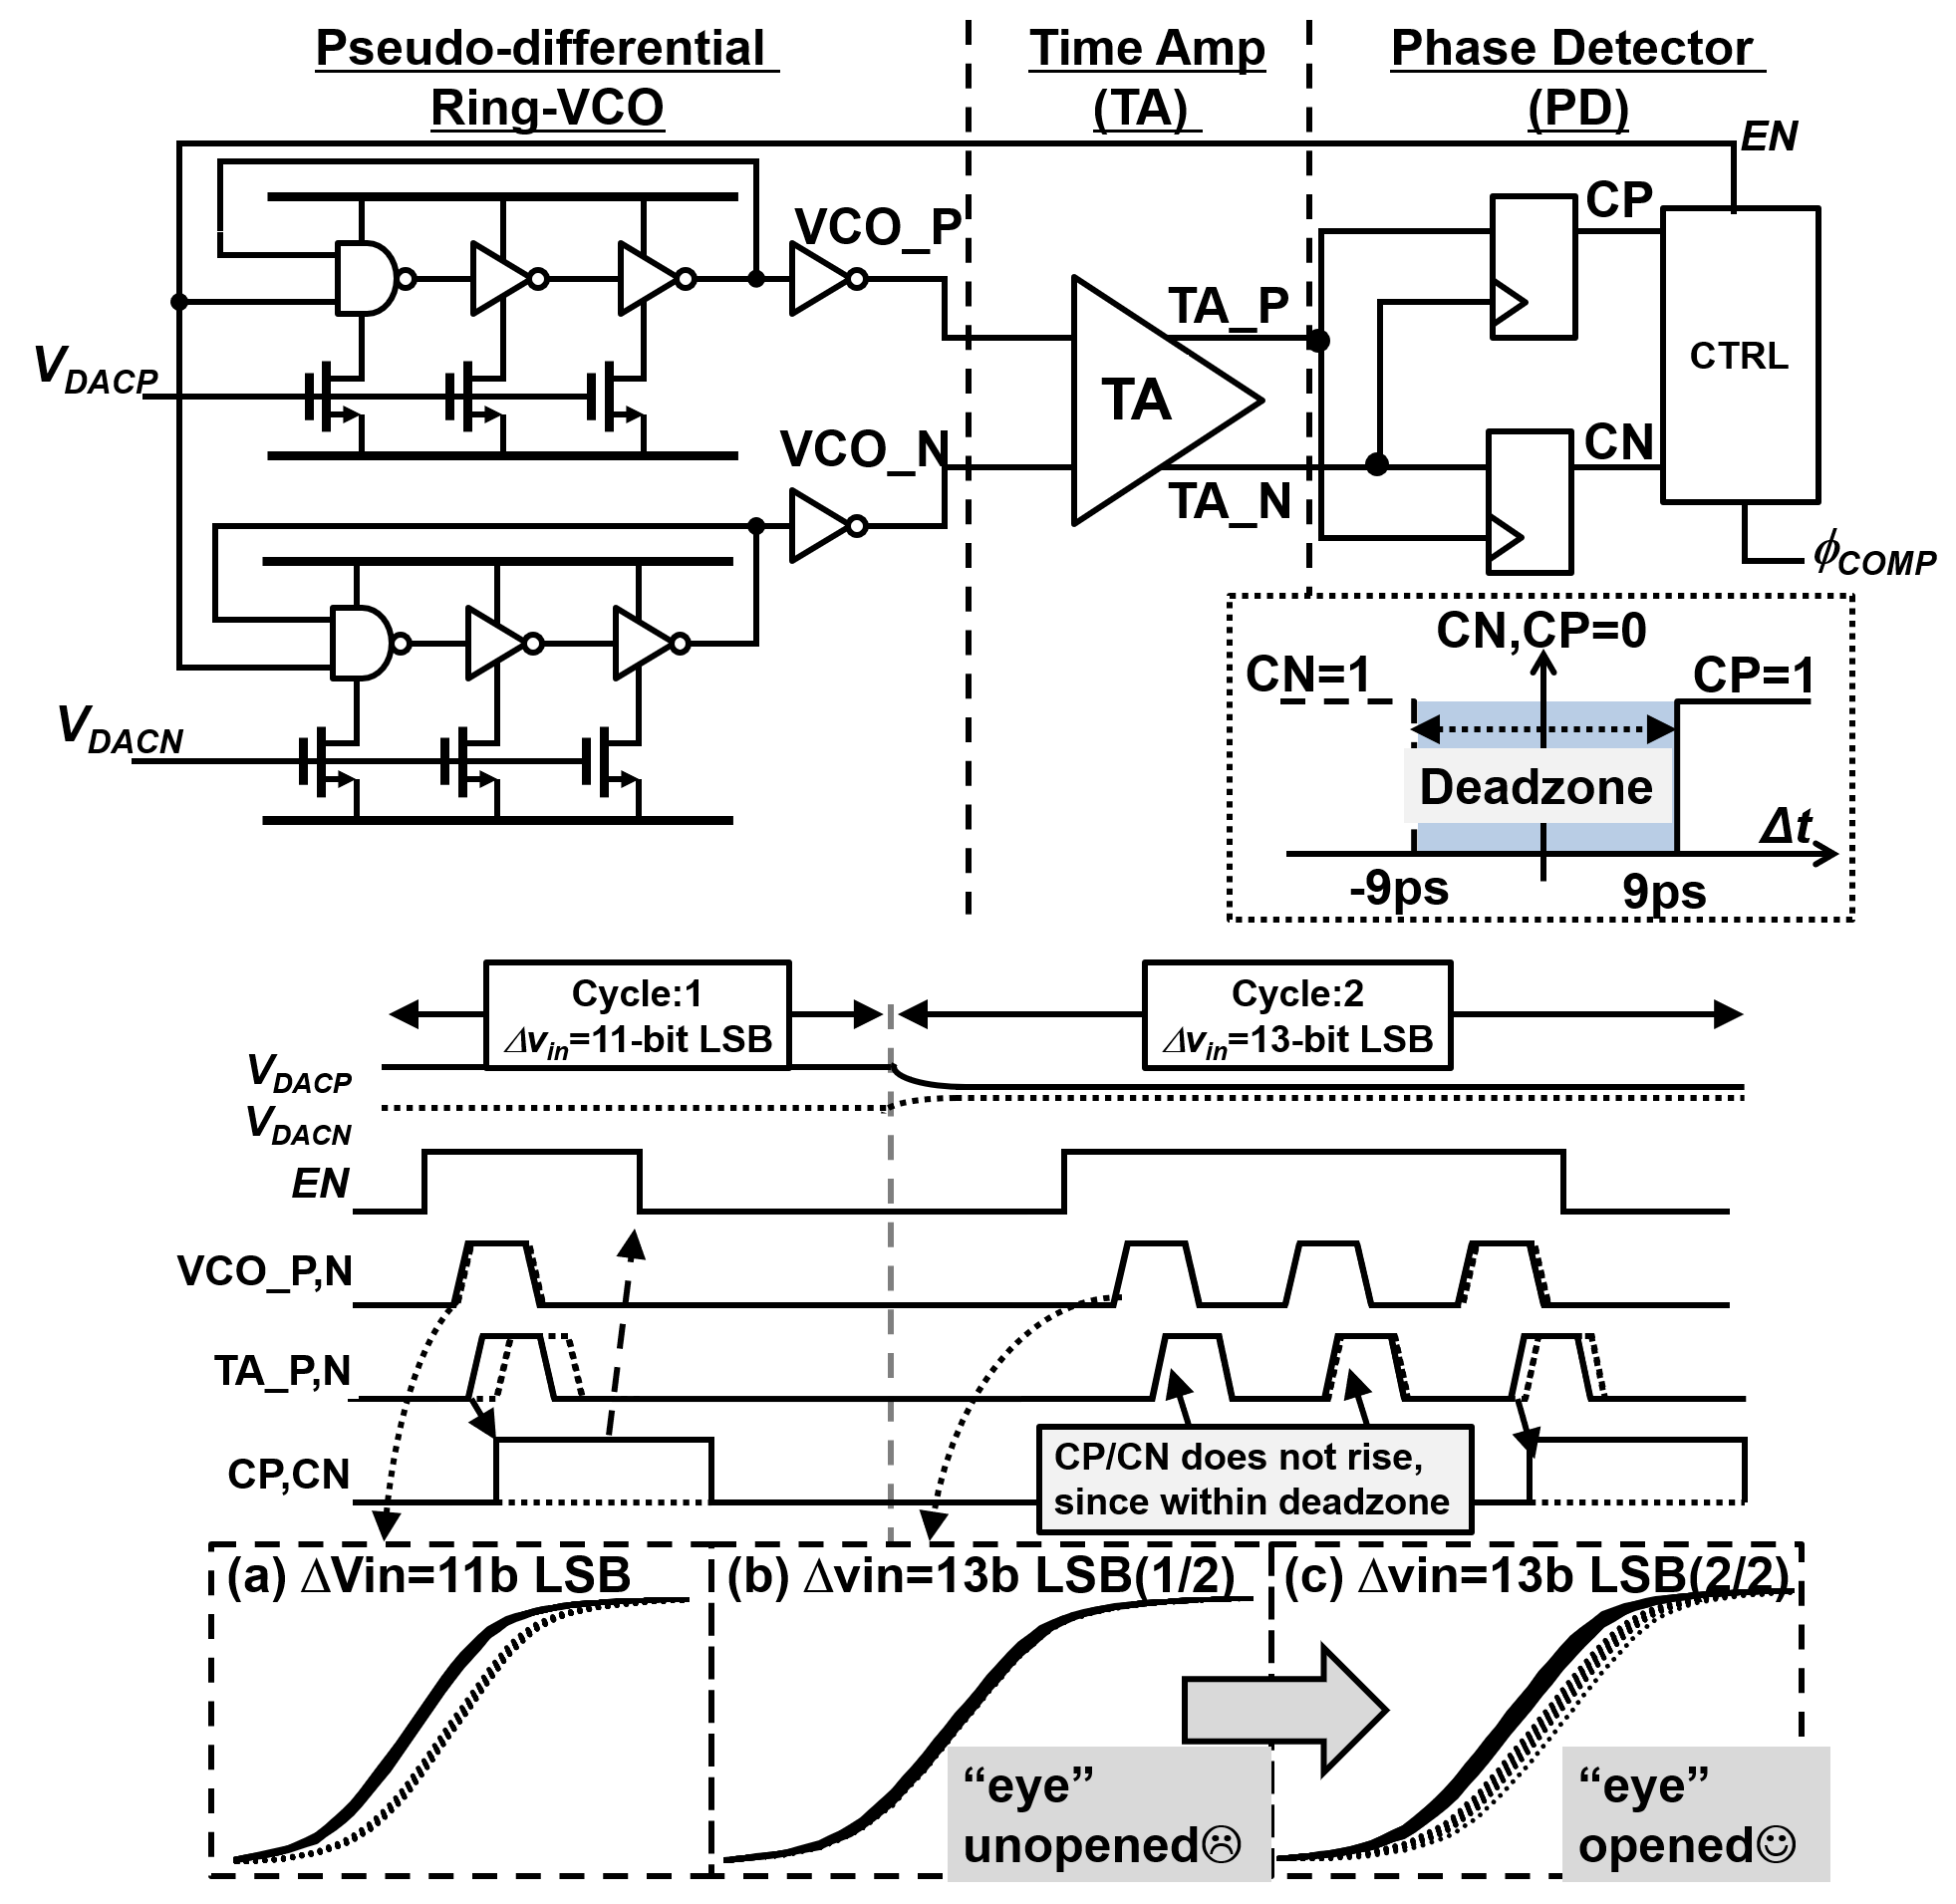
\includegraphics[width=0.5\textwidth]{figs/fig4.png}
  \captionsetup{font=footnotesize}
  \caption{\textbf{ADC}}
  \label{highlight}
\end{figure}
我々は入力電圧差に応じノイズモードを自動的に切り替えるVCOベース比較器を提案する\cite{yoshioka201413b}。VCO比較器は入力電圧差に応じたノイズレベルで動作し消費電力もスケールする。そのためVCO比較器のSAR動作中の電力は:(式)

となり2つのノイズモード切り替えを行うDDNR比較器と比べ比較器電力を半分に削減することができる。

Fig.3 shows the schematic of VCO based comparator. Similar to the delay-line based comparator \cite{agnes20089}, the input analog voltages are given to control the slew rate of ring oscillator cell. Therefore, the ring oscillator oscillating frequency is decided by the input analog voltage (VinP or VinN). To relax the phase detector operation, the VCO outputs ($VCO_P$, $VCO_N$) are connected to a time amplifier (TA). TA \cite{lee20089} is used to amplify the “time” difference between the two input pulses and in this design, the gain is set to 8. Finally, the outputs of TA ($TA_P$, $TA,N$) are connected to the phase detector.

Fig.4 shows the VCO comparator operation in the case of large and small D*vin*, respectively. In this example, at cycle 1, D*vin* is fairly large (> 4 LSB), and proposed comparator operates as a delay-line comparator. When *ACT* rises, the VCOs are “enabled” and pulses start to travel through the ring-VCO cells. The pulses reach the TA and their time difference is amplified. In this case, $TA_P$ clearly rises faster than $TA_N$ and the D-FF based phase detector outputs the comparison results of CP=1 and CN=0. Once the comparison results are obtained, *ACT* is set down to “disable” ring-VCO and unnecessary oscillation is prevented.

Next, the comparator operation with small D*vin* (Cycle 2 in Fig.4) is explained. Similarly, *ACT* rise and the pulses transmit through the VCOs. Fig.4(a) and (b) plot the VCO outputs of 50-times noise simulation with D*vin* of 4 and 1 LSB respectively. Note that in (b), an “eye” is not opened because jitter is larger than the input signal dependent time deference. In such conditions, the comparator cannot make a correct decision and noise reduction operation is required.

In this circuit, event of small D*vin* is easily detected by effectively utilizing the “dead zone” of the phase detector designed with standard logic D-FF cell. In this work, the dead zone for typical condition is 9 ps. The effect of PVT will be discussed later. If the time difference of pulses is small and within the dead zone, the phase detector does not generate any output signal. Interestingly, since the VCOs are “enabled” during these events, the pulses of the second oscillation cycle are then transmitted. The same procedures continue until the pulse time difference is large enough to exceed the dead zone. In Fig.4, the TA output pulse exceeds the dead zone after 3 oscillations and comparison results are obtained and *ACT* sets down. Fig.4(c) shows the noise simulation of VCO output after 3 oscillations and “eye-opening” is clearly observed. By this eye-opening oscillation, the VCO comparator adaptively reduces noise when vin is small.

\subsection{Noise Analysis of VCO Comparators}
\begin{figure}[ht!]
\centering
 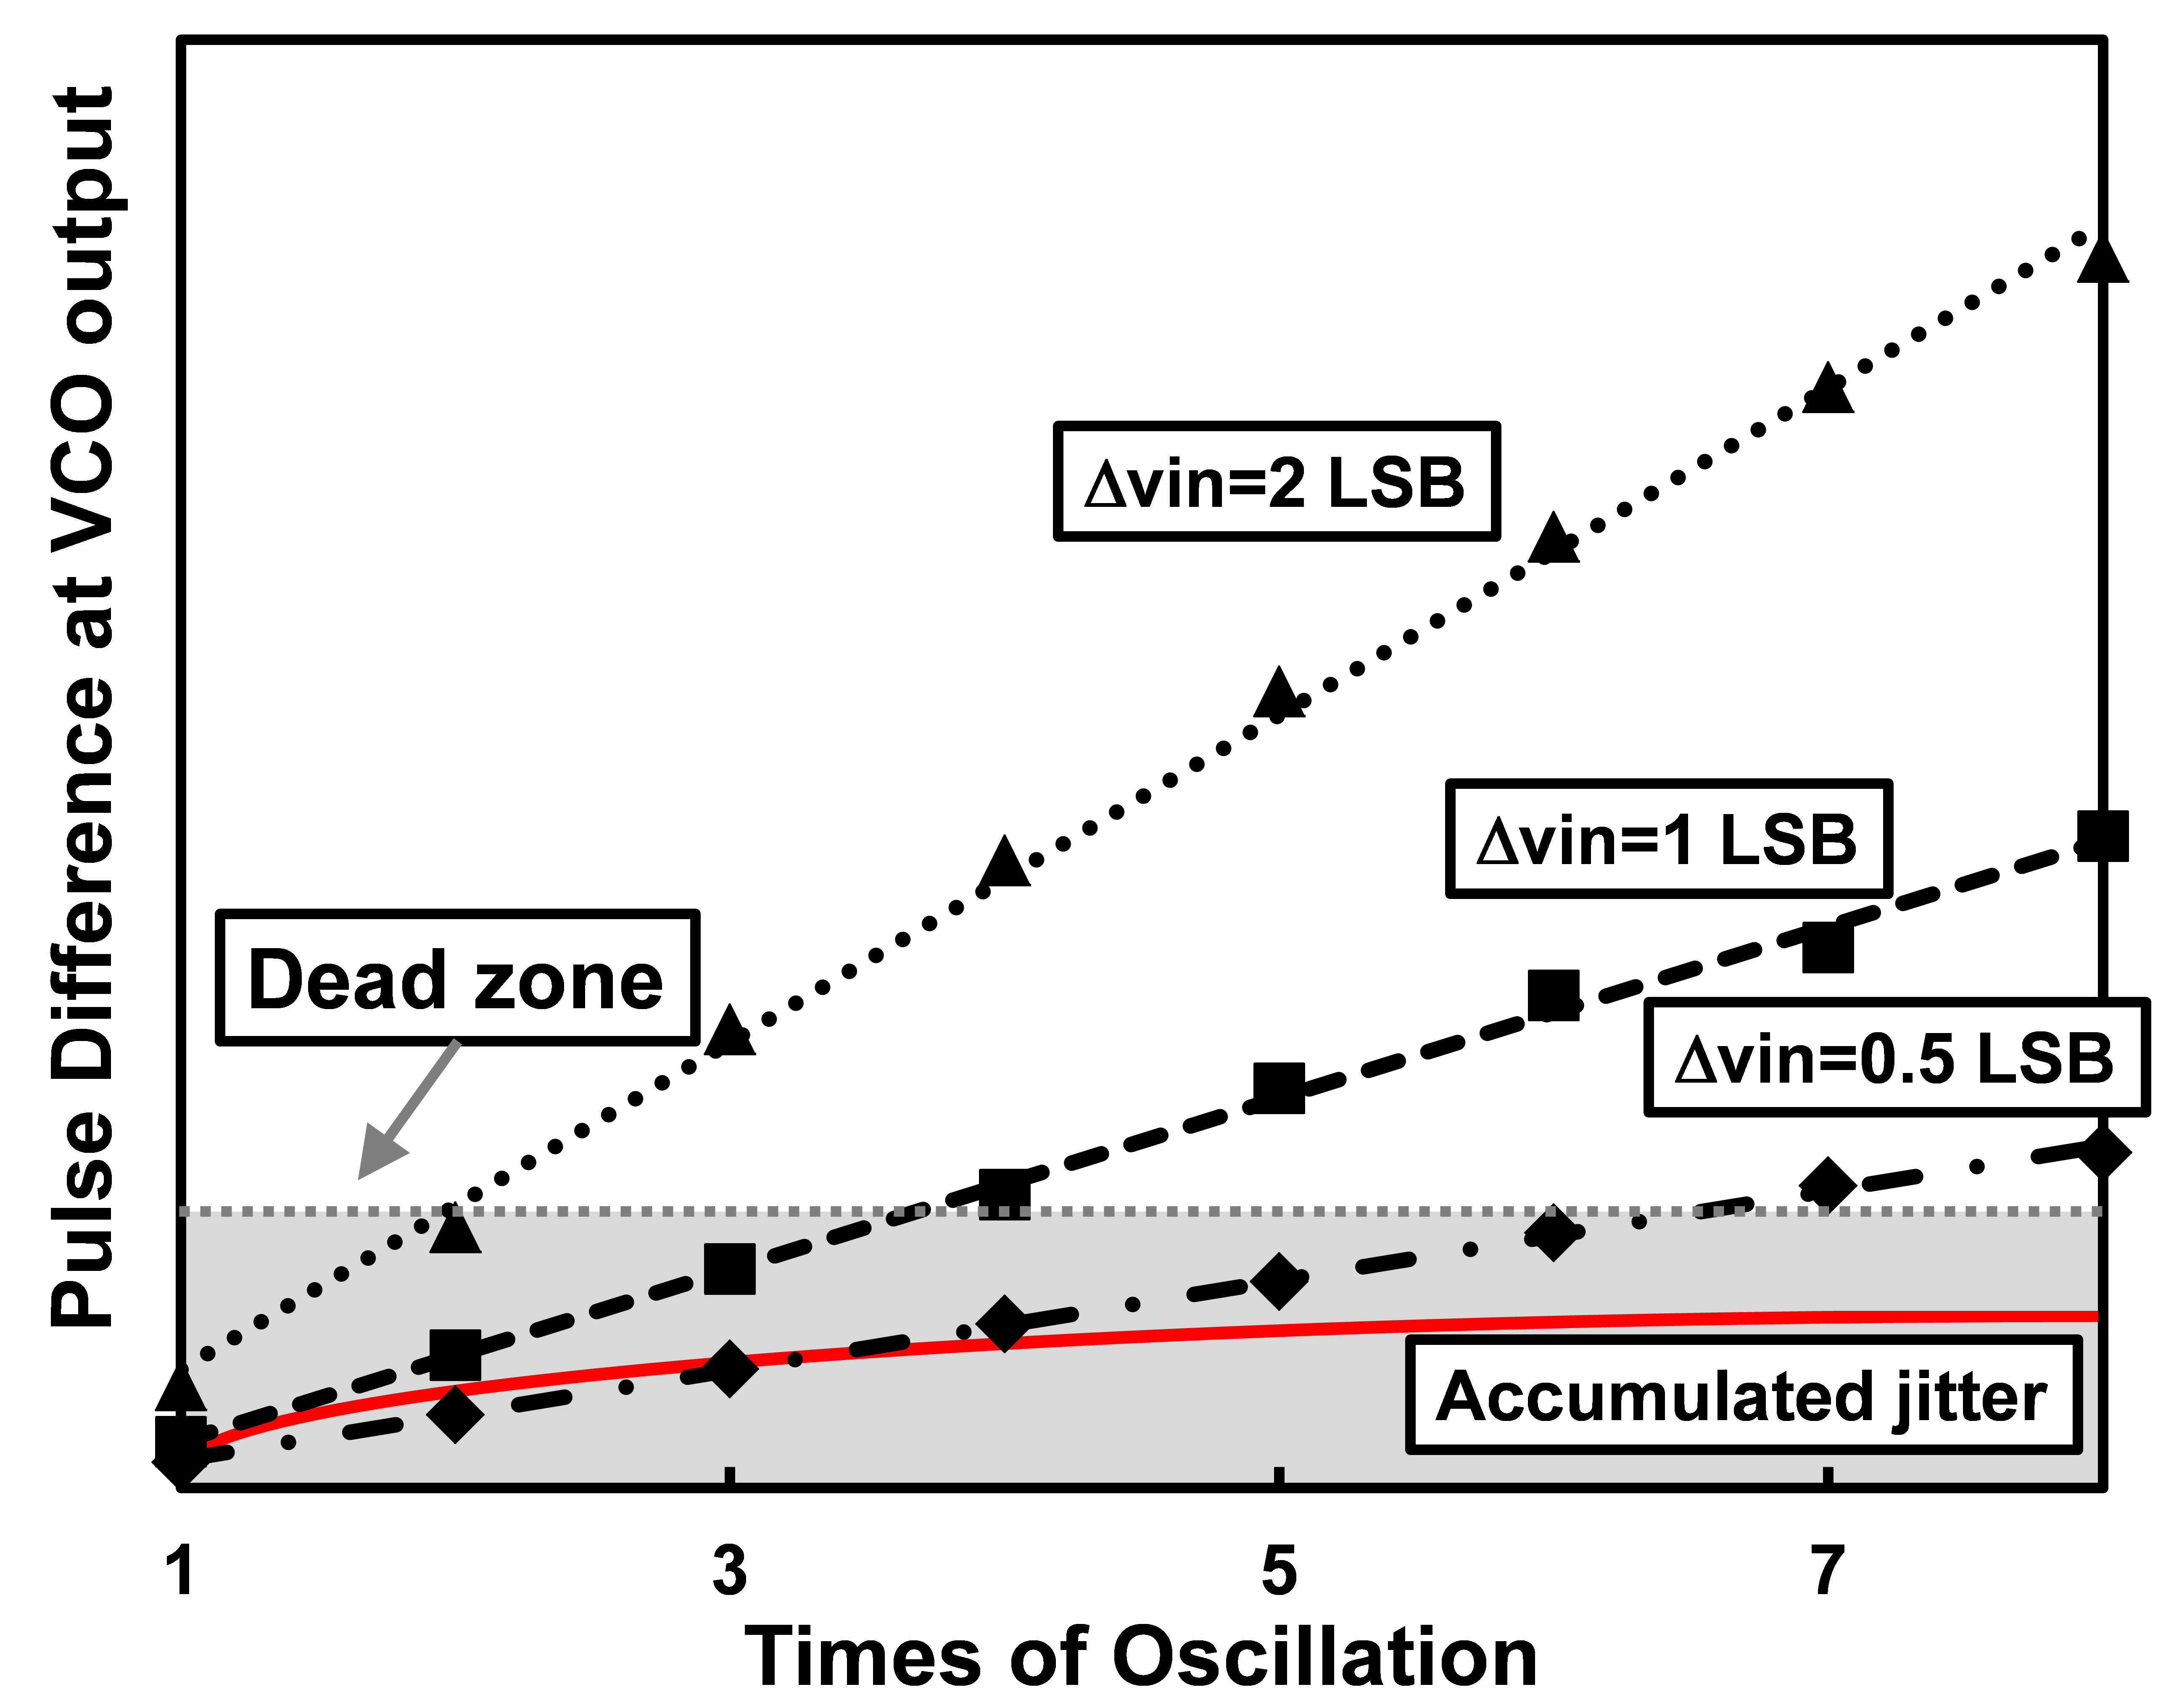
\includegraphics[width=0.5\textwidth]{figs/fig5.png}
  \captionsetup{font=footnotesize}
  \caption{\textbf{ADC}}
  \label{highlight}
\end{figure}
Further analysis of the eye-opening oscillation is given in the following. In Fig.5, the simulated the eye-opening oscillation is given. In Fig.5, the simulated oscillation count times (N) versus pulse difference is plotted for dvin of 10.5, 12, and 24 LSB respectively. We can observe that oscillation times and pulse difference has a linear relationship of sqrtN and ?? is decided by dvin. On the other hand, the accumulated jitter is in proportion to square root of 発振時間 or sqrt(N) \cite{hajimiri1999jitter,abidi2006phase}. In the case of dvin is 1 0.5 LSB, even though the jitter may be dominant at 1-3 times of oscillation, the signal dependent pulse difference will become dominant as the number of oscillation increase. The area in gray indicates the dead zone and as long as the pulse difference is under that value, oscillation will continue. Therefore, for dvin=0.5, 1, and 21, 2, and 4 LSB, we can guarantee accurate comparison results. However, to prevent meta-stability when dvin<0.25 LSB, the maximum oscillation N is was set to 8 in this design.

VCO比較器のノイズはref.\cite{luo2020input}で詳しく議論されているため詳しい導出は行わないが今後の議論に関わるVCO比較器のノイズを決定する重要なデザインパラメータ(インバータステージ数、dt、テールトランジスタW/L)について明確化する。VCO比較器の基本的なノイズ特性はノイズ源を白色雑音と仮定するとリング発振器VCOと同等でありref.\cite{hajimiri1999jitter}の解析結果をそのまま活用できる。VCO比較器ではリング発振器のショートタームジッタが比較器ノイズとして現れる。そのためIRNは\cite{hajimiri1999jitter}で解析されている通りリングのインバータ数のsquare rootに反比例する。また比較は時間差がデットダイム(デルタt)を超えるまでは発振動作が繰り返されるため、IRNは同様にデルタtにも反比例する。

リングVCOのジッタと異なるのはVCO発振器は電圧から時間への変換器も兼ねている点である。そのためkVCOが大きければ大きいほどジッタに対する耐性(signal dependantの成分)が向上するためIRNは向上。これはテールトランジスタのW/Lによって決定づけられ、IRNは反比例する。

まとめると。。

IRN = Njitter/(G*sqrt(N)*dT)

また比較毎にリングオシレータの位相はリセットされる。そのため位相雑音にはハイパス特性がかかるため、1/f雑音といったロングタームジッタについては考慮しなくても良い。

\subsection{Power Saving Characteristics}
提案したVCO比較器は入力レベルに応じたエネルギーを消費する。まず特性を確認するため、入力差を振ったシミュレーション結果のVdif vs Energyをプロット。

VCO比較器はノイズをかんたんにプログラム可能。上記IRNは理論限界

10, 10.5, 11, 11.5, 12, 12.5, 13, 13.5

low noise vs ddnr vs vco comp.

10bit comparator

\subsection{PVT drift resistance}
式IRNを見るとG, Nは設計アーキテクチャとして決定。ジッタはPVT依存性があり、dTをジッタと逆方向に変動させられればIRNをPVTを通し一定に保つ。

我々のVCOはタイムアンプのgm依存性を利用し、PVTを通しノイズ一定化する。

Next, PVT variation effect to comparator IRN is discussed. Firstly variation effects at fast corners such as lower VTH, reduced temperature, and increase of power supply are considered. This will increase the bandwidth of VCO cells and increase the jitter as well. However, the TA gain will decrease since it is proportional to 1/gm. Interestingly, this cancels the effect of VCO jitter increase because more oscillation will be required to exceed the dead zone. Although, the overall IRN degrades a little since the dead zone decreases by 10%. Similarly, VCO jitter decrease when VTH rises and TA gain increase as well, cancelling each other. IRN improves slightly since the dead zone expands.

PVT versus ENOB シミュレーション

IRN = Njitter/effdead

FF条件では熱雑音やバンド幅増加のためNjitterは増加。一方でタイムアンプのゲインは1/gmに比例する。するとVCOから見た実行的なdeadzoneはタイムアンプゲインをA、DFFのdeadzoneをtdeadzoneとすると

Effective deadzone = deadzone/A

シミュレーション結果の図。

FF条件では1.5倍Effdeadzoneが増加し、Njitterの増加分をキャンセルし比較器としてのIRNを一定に留める。その代わりVCOは判定するのにより発振が必要となり、消費電力は増加する。
またSS条件ではEffdeadzoneは0.7倍に縮小する。この環境ではNjitterも低減するため、トータルとして比較器IRNは一定にとどめられる。
このようにタイムアンプを用いたVCOはPVTを通じノイズを一定に留めるような効果を内在する。その代わりトレードするのは消費電力と比較時間。

派生した他研究のVCO比較器はタイムアンプを用いず、比較電力自体は我々のものよりも小さくできる。一方でこのようなPVTに対するノイズキャンセル効果は持たない。

タイムアンプは比較器のエネルギーの1/3を消費する。残り2/3はほぼVCOであり、デジタルロジックは10%ほどの電力。

\section{Circuit Implementations}
\subsection{13-bit SAR ADC implementation}

\begin{figure*}[ht!]
\centering
 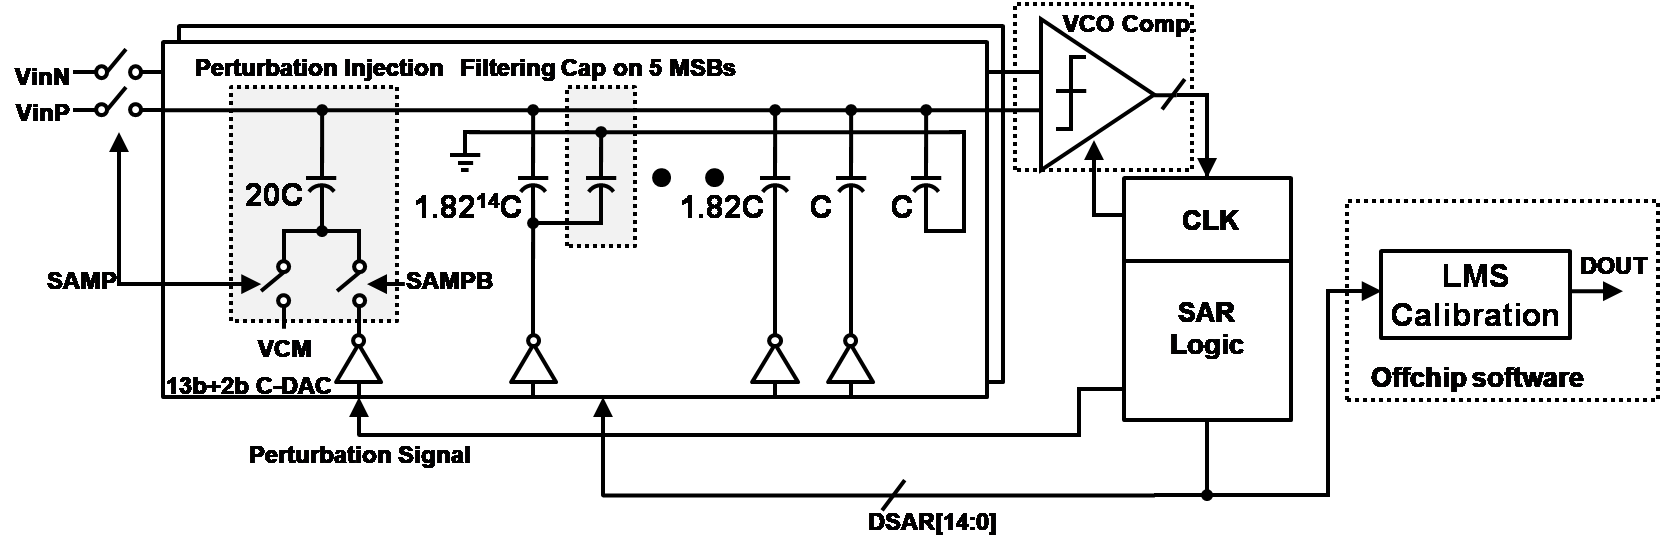
\includegraphics[width=1\textwidth]{figs/fig7.png}
  \captionsetup{font=footnotesize}
  \caption{\textbf{ADC}}
  \label{highlight}
\end{figure*}

高精度なVCO比較器を実証するため、13bitの低電力SAR ADCを設計する。
The entire 13b SAR ADC architecture is shown in Fig.7. C-DACの電力をできるだけ低減するため、ref.\cite{liu201012b}と同様の sub-binary C-DAC and perturbation logic for LMS calibrationを用いる. The C-DAC has 2b redundancy and has a sub-binary radix of 213/15=1.82. To suppress the noise of C-DAC buffers, filtering capacitors \cite{miki20154} are provided until 5th bit from MSB. Unit capacitor (C) of 0.5fF was chosen  to meet kT/C noise requirements.

To cancel the capacitor mismatch effect, perturbation based digital calibration \cite{liu201012b} is employed. When the calibration is active, two conversions are resolved for a same sample. The conversions are perturbed with offset of ±Δinjected before the SA cycle starts. The perturbation injecting capacitor is 20C as shown in Fig.7. After the first conversion ends, the perturbation signal is inverted so that it will inject with different polarity. The LMS calibration engine was implemented off-chip.

\subsection{VCO Comparator with multiple noise modes}
\begin{figure}[ht!]
\centering
 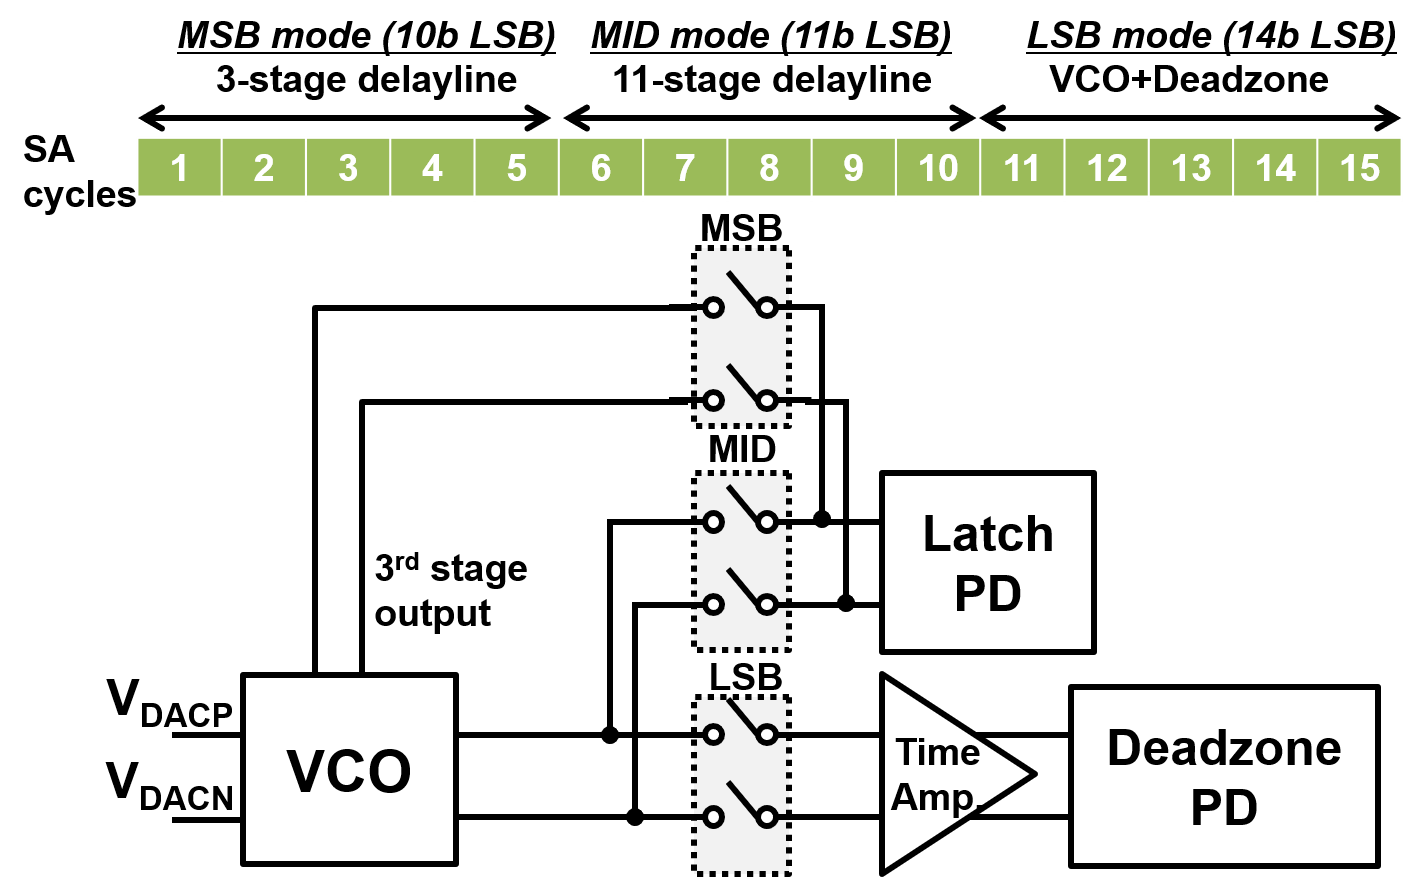
\includegraphics[width=0.5\textwidth]{figs/vco-entire-r1.png}
  \label{highlight}
\end{figure}

高精度SAR ADCではセトリングなどの影響を緩和するため冗長性込で設計することが多い。
今回の13-bit SAR ADCもsub-binary radixであり2bitの冗長性をもたせている。
このようなsub-binary SAR ADCではbit毎に冗長性が割り当てられ、各bitに判定エラーが含まれても後段のfine比較が精微であれば全体として精度劣化は起きない。例えば今回の設計では上位5bitでは200 LSB相当の判定エラーを許容でき、上位ビットにおいてsub-LSB精度を持つVCO comparatorを用いるのはオーバースペック。

我々は複数のノイズ性能を可変にできるVCO比較器を提案する。(すケマ)
アイデアとしてはdelay line comparatorと発振を行うVCO比較器と動作を切り替えることでノイズパフォーマンスと消費電力をスケールすること。
少ない面積と簡単なスイッチング回路でVCO比較器に3つのノイズモードをもたせる。

上位5SA。MSBモード:単純な3-stage delay lineとして動作。判定エラーを許容できる上位比較。 IRN:2mVpp
中間5 SA。MIDモード:11-stage delay lineとして動作。 IRN:xxxuVpp
下位5SA。LSBモード:2章で記述した11-stage VCO動作。IRN:80uVpp

MSB,MidではDeadzoneを用いたPhaseDetectorで判定せず、ラッチベースのPhaseDetectorで強制的に判定結果を取得。

\subsection{VCO and Time Amp. designs}
\begin{figure}[ht!]
\centering
 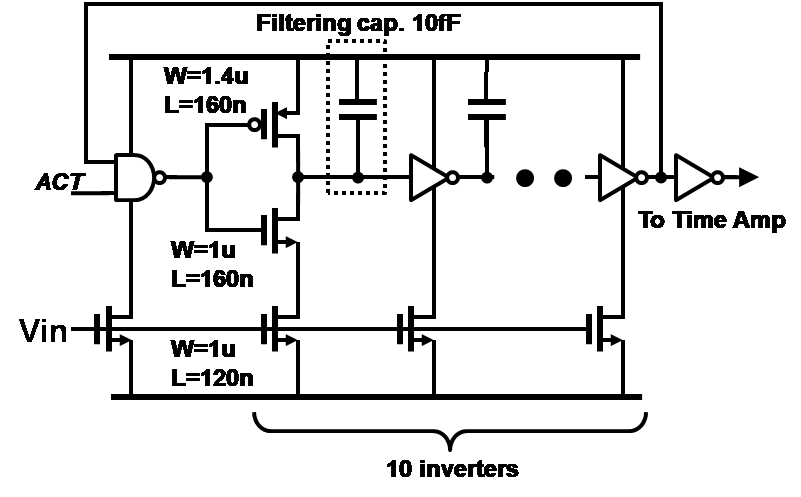
\includegraphics[width=0.5\textwidth]{figs/fig6.png}
  \captionsetup{font=footnotesize}
  \caption{\textbf{ADC}}
  \label{highlight}
\end{figure}

\begin{figure}[ht!]
\centering
 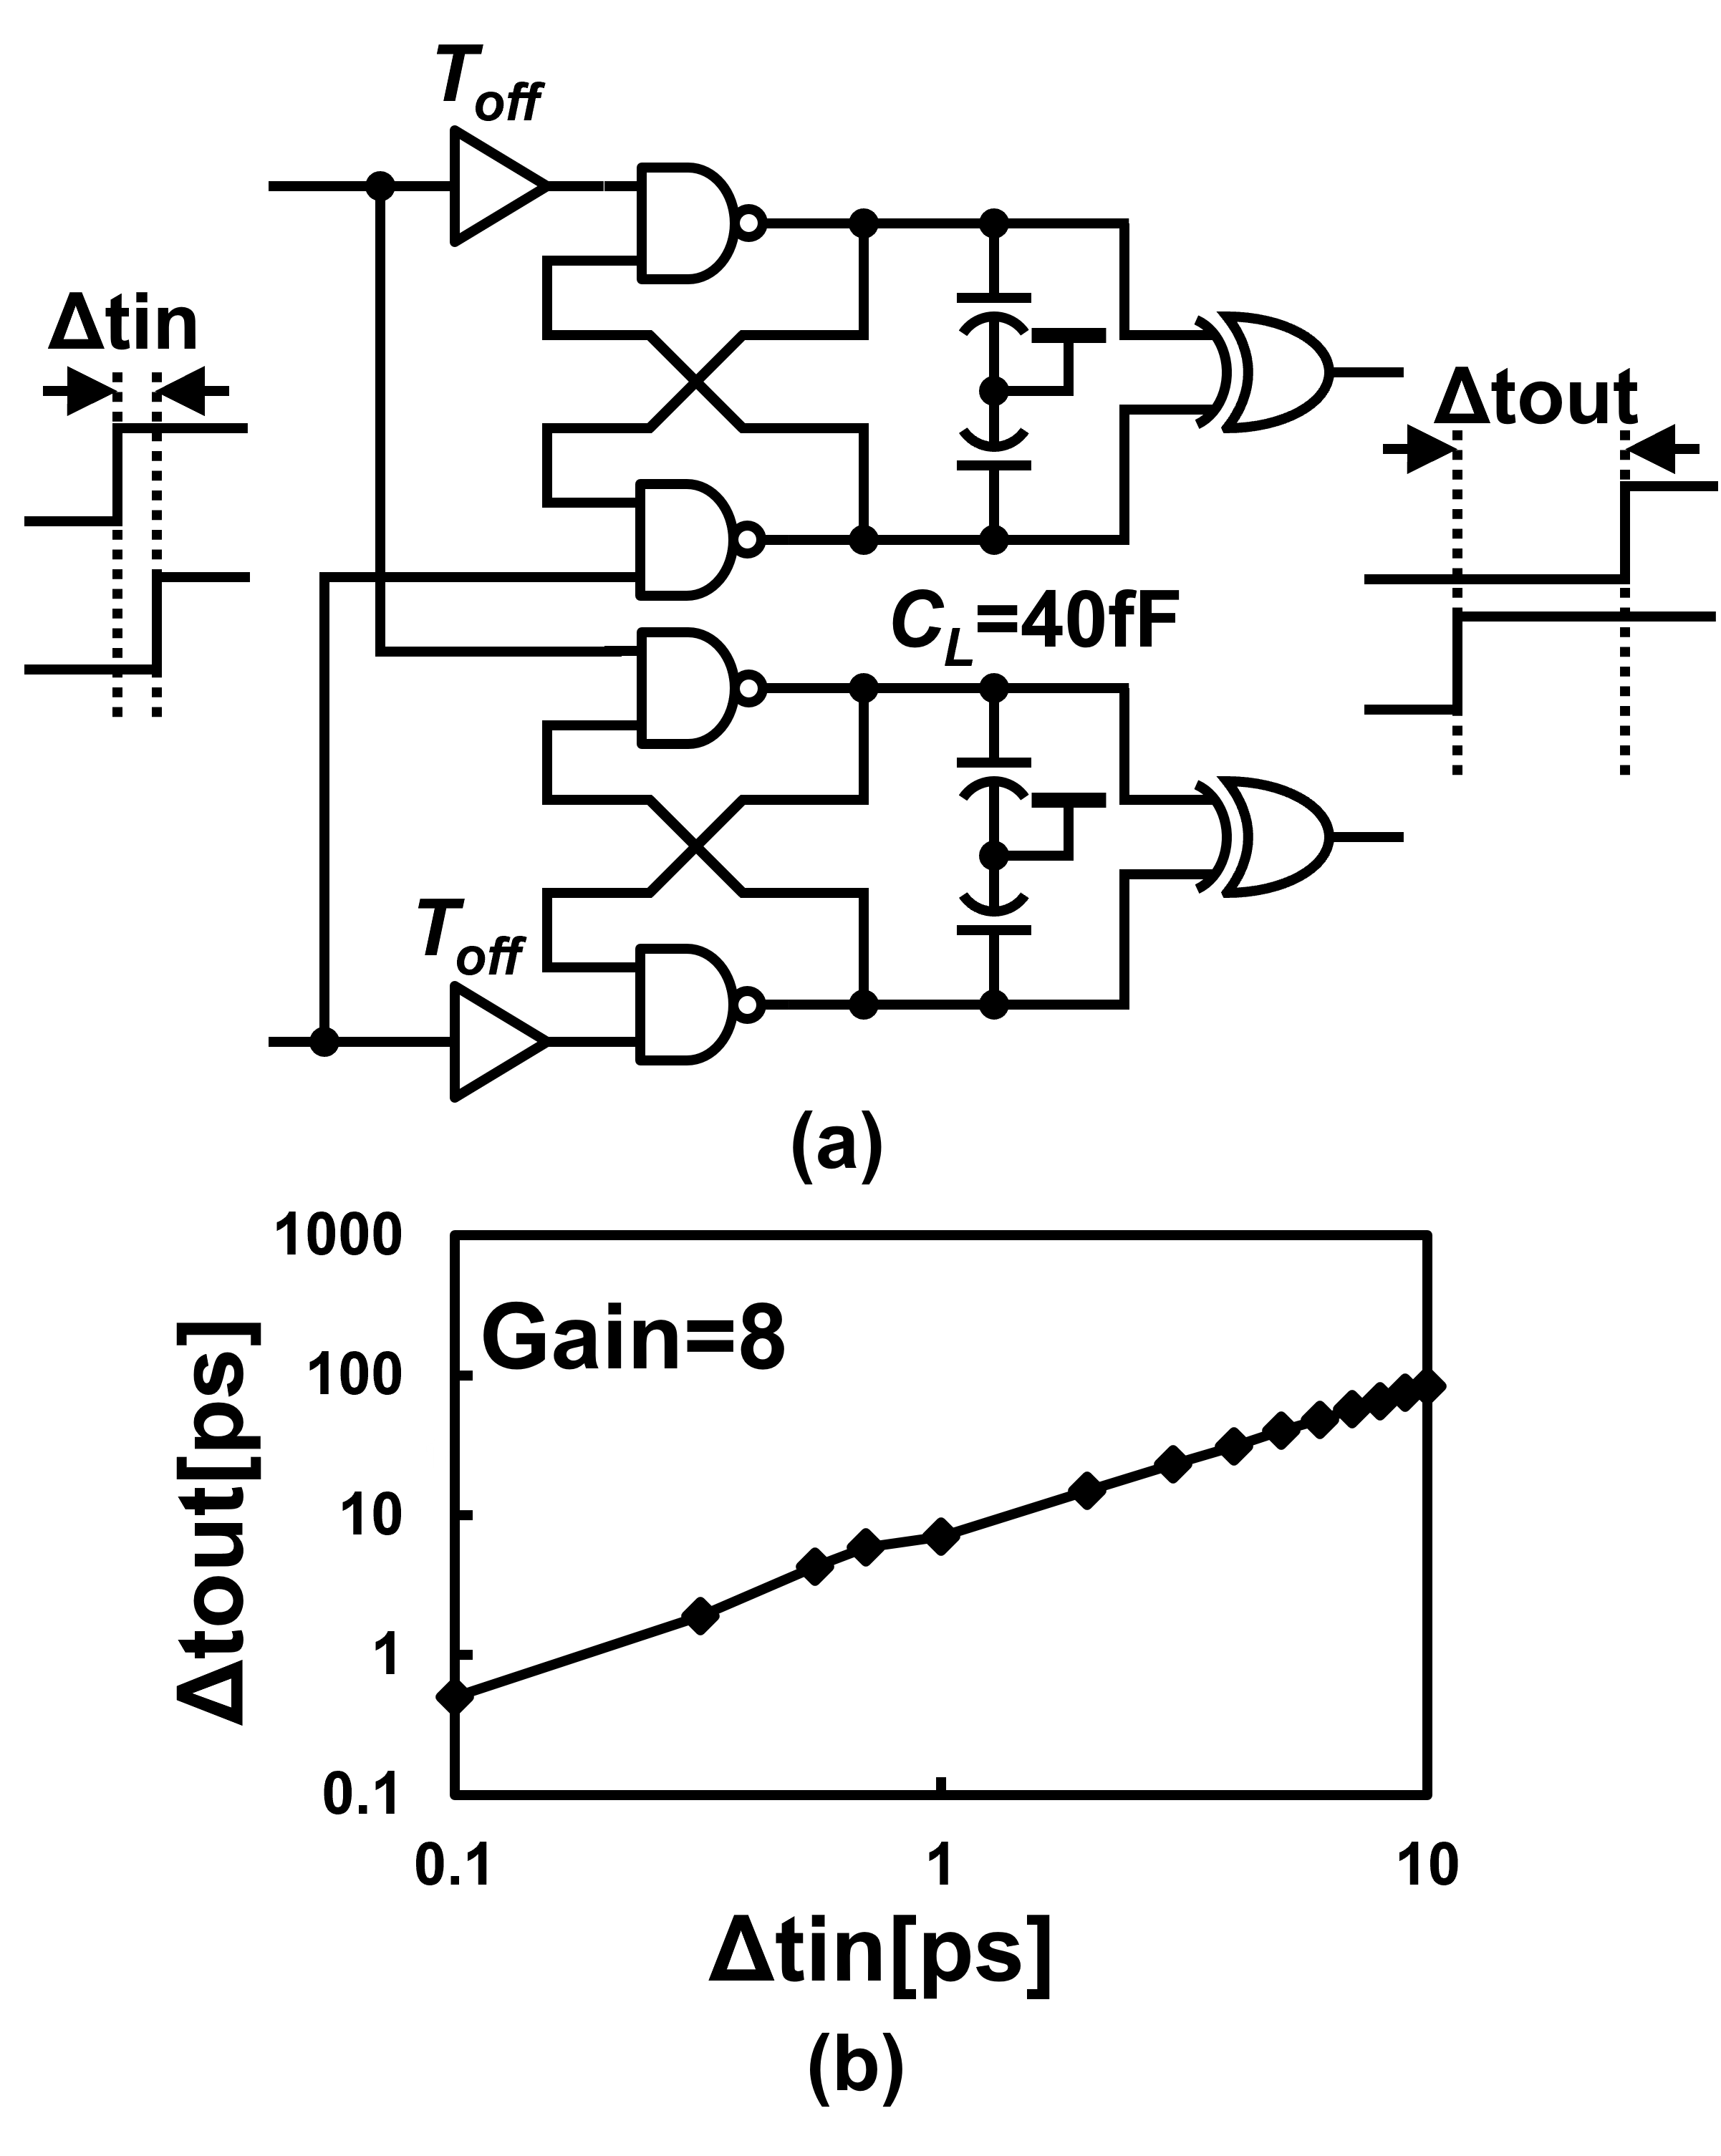
\includegraphics[width=0.5\textwidth]{figs/ta_chara.png}
  \captionsetup{font=footnotesize}
  \caption{\textbf{ADC}}
  \label{highlight}
\end{figure}


\section{Experiment Results}
\begin{figure}[ht!]
\centering
 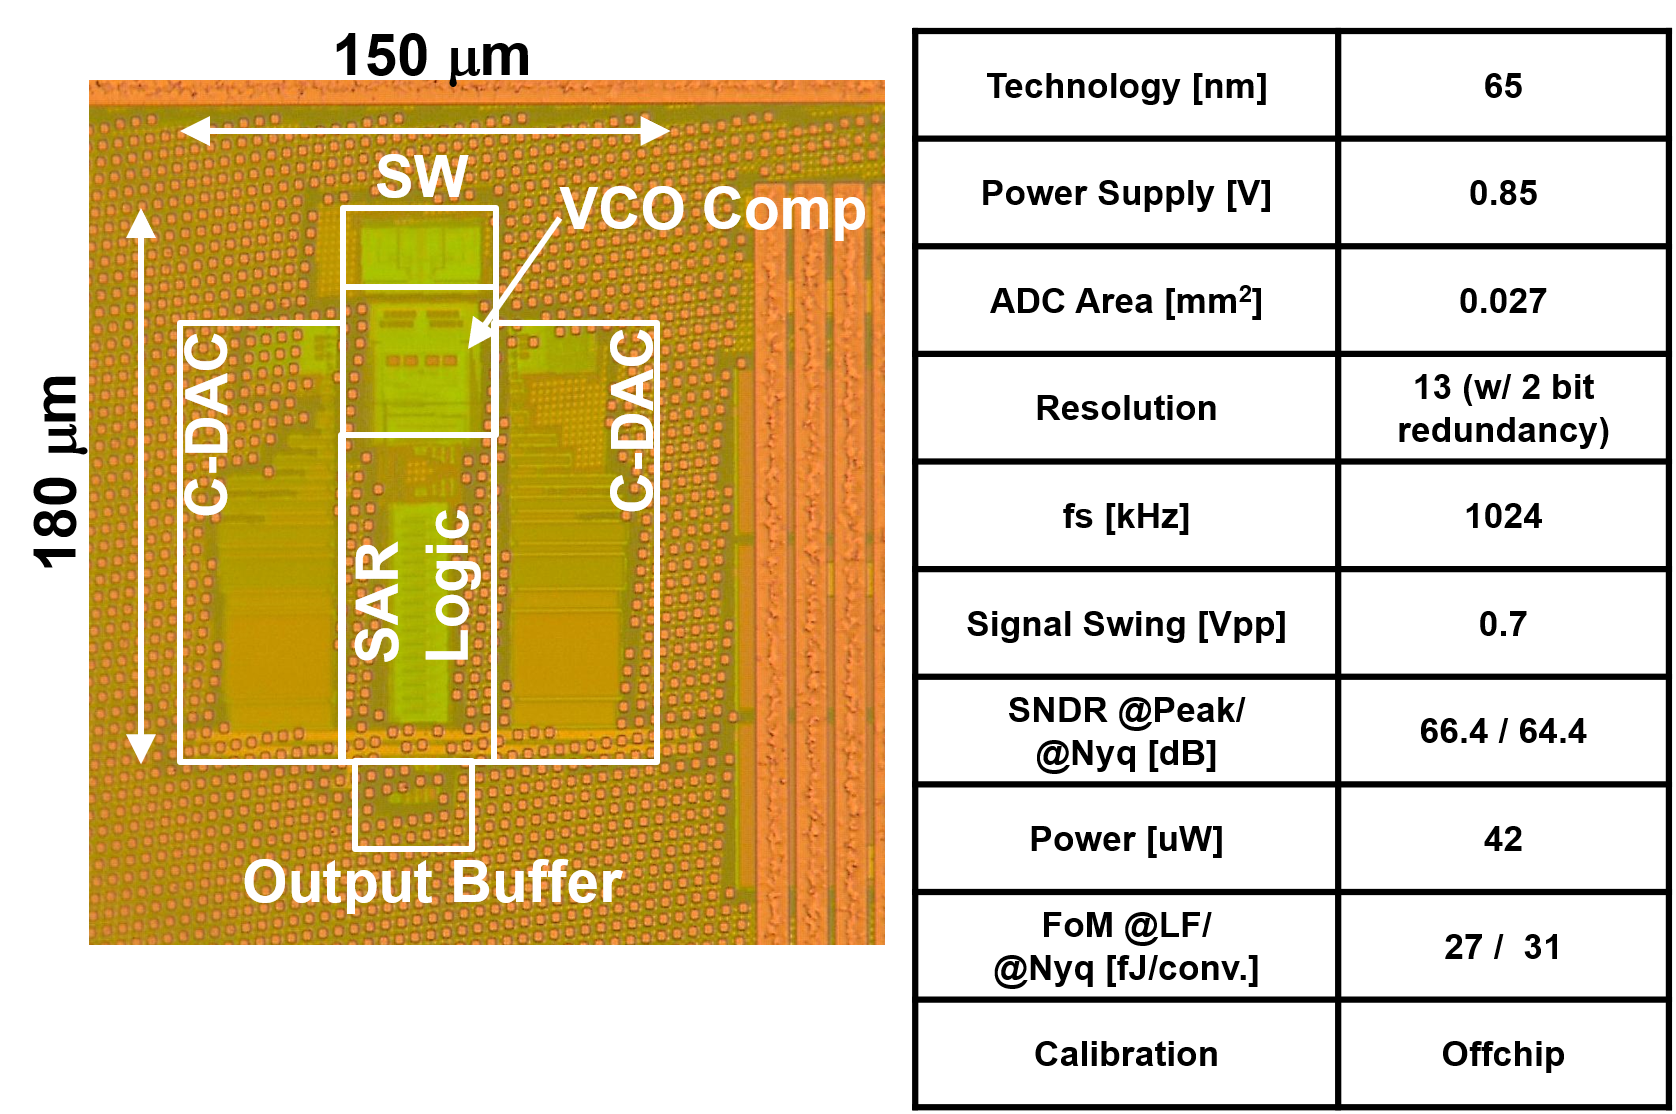
\includegraphics[width=0.5\textwidth]{figs/chipphoto.png}
  \captionsetup{font=footnotesize}
  \caption{\textbf{ADC}}
  \label{highlight}
\end{figure}

\begin{figure}[ht!]
\centering
 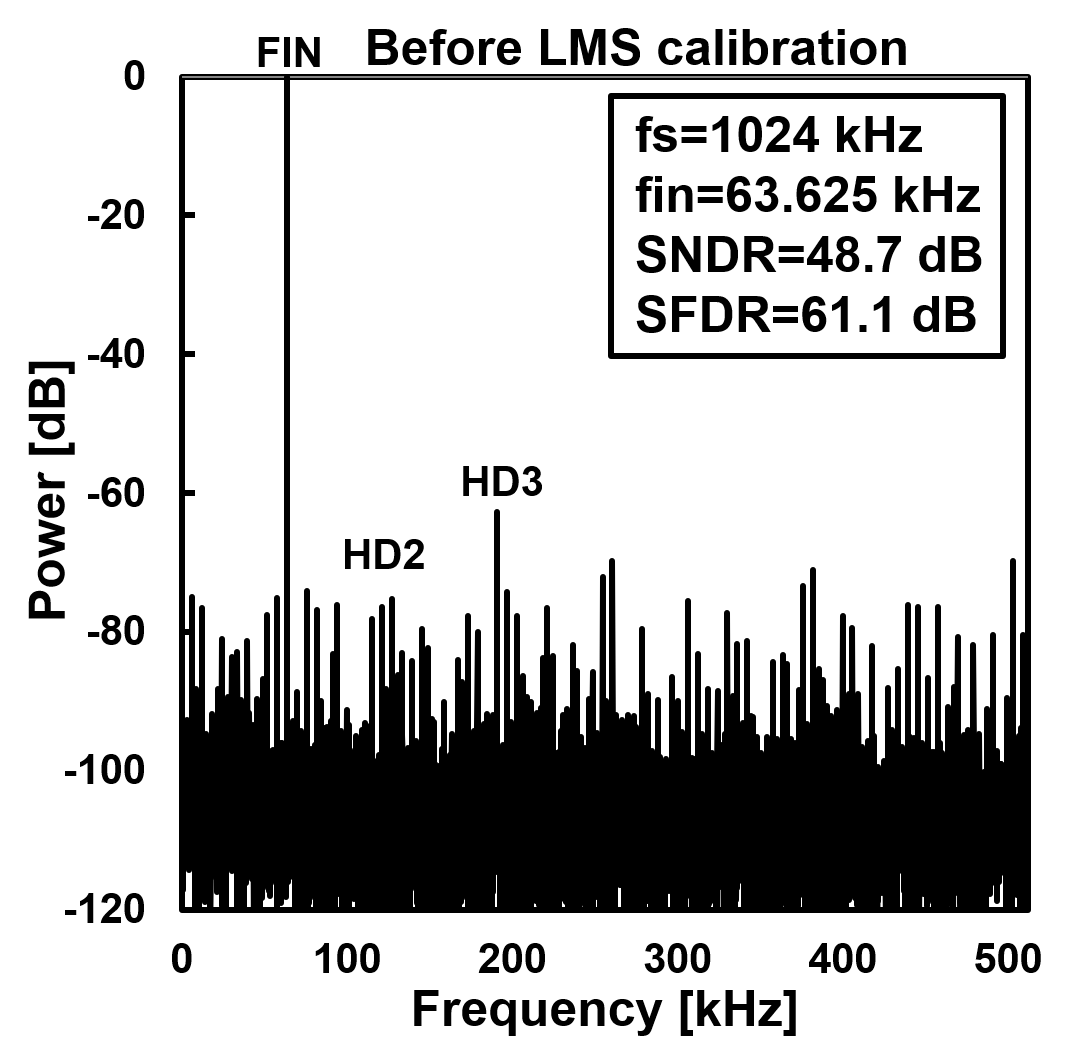
\includegraphics[width=0.5\textwidth]{figs/beforecal.png}
  \captionsetup{font=footnotesize}
  \caption{\textbf{ADC}}
  \label{highlight}
\end{figure}

\begin{figure}[ht!]
\centering
 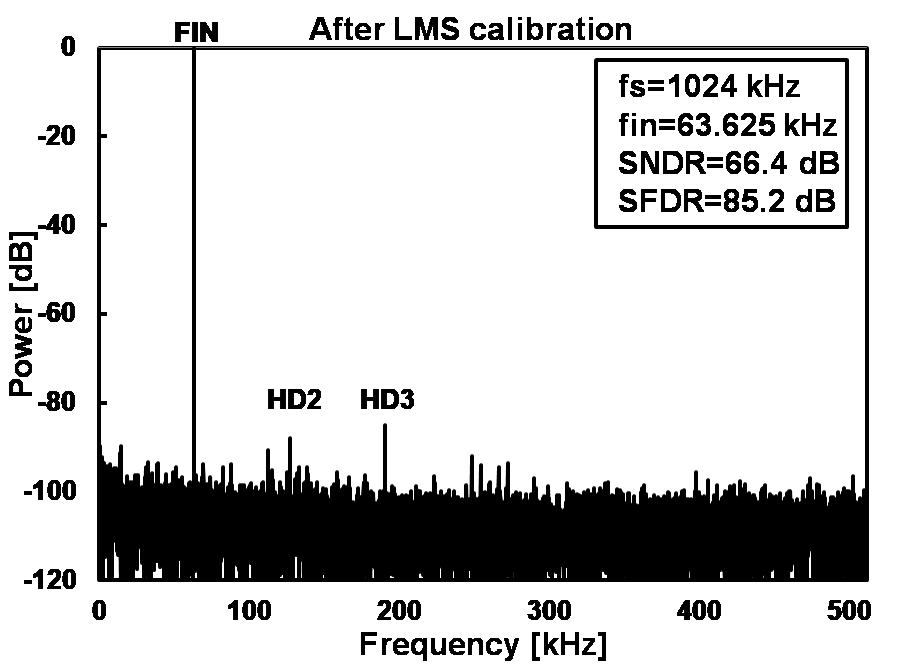
\includegraphics[width=0.5\textwidth]{figs/aftercal.png}
  \captionsetup{font=footnotesize}
  \caption{\textbf{ADC}}
  \label{highlight}
\end{figure}

\begin{figure}[ht!]
\centering
 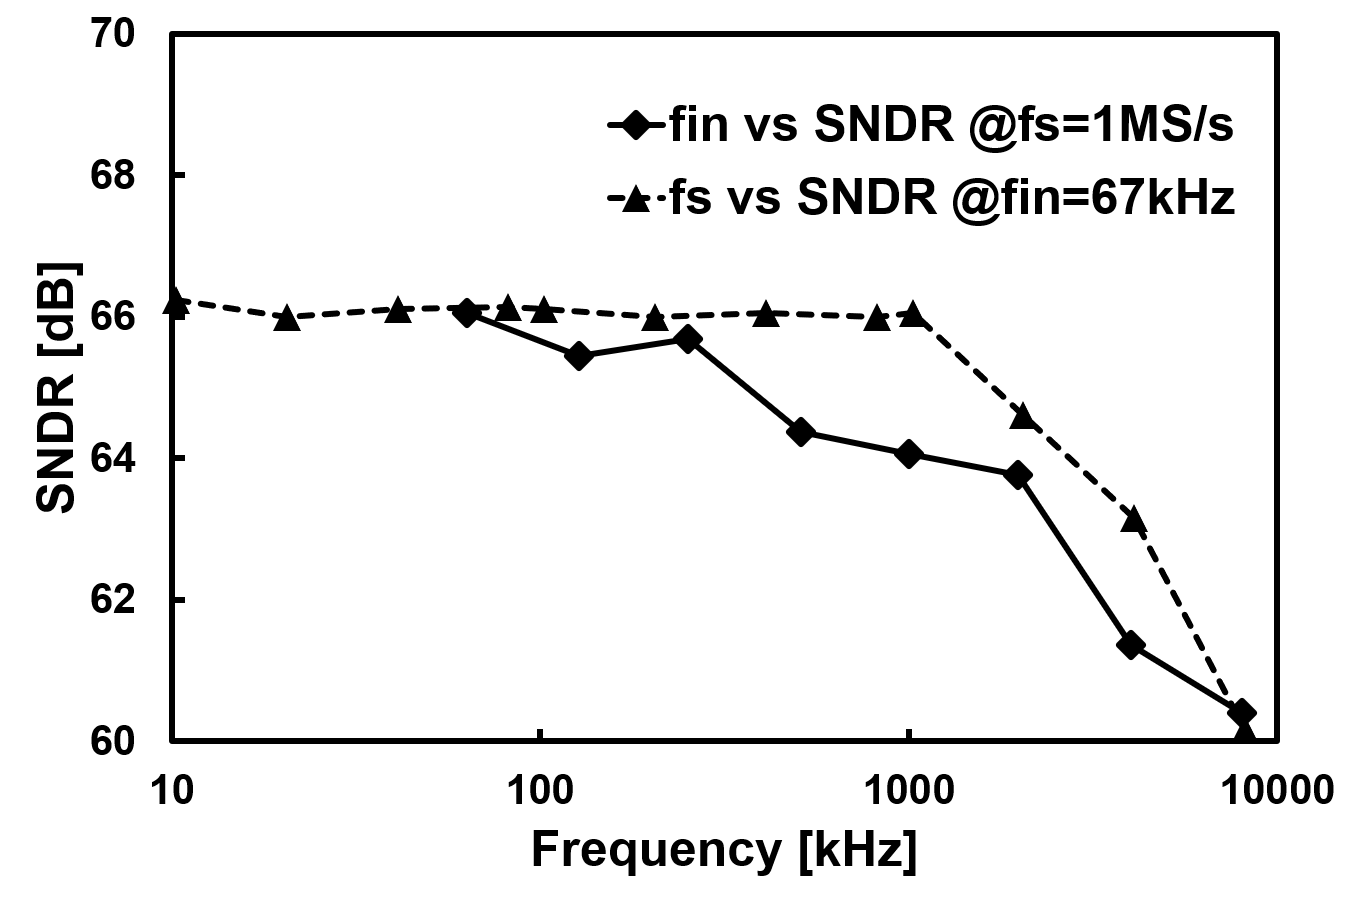
\includegraphics[width=0.5\textwidth]{figs/freq-sndr.png}
  \captionsetup{font=footnotesize}
  \caption{\textbf{ADC}}
  \label{highlight}
\end{figure}

The SAR ADC was fabricated in 65-nm CMOS and Fig.8 shows the chip micrograph and a performance summary. 
Fig.9 shows a result of 16384-FFT before and after LMS calibration. The two FFT results were lead using the same raw data, but different bit weighting were used: weighting used in schematic and weighting derived via calibration. Therefore, noise situation is exactly the same. Even though no trimming to the comparator was carried out, fine noise performance was achieved. Even with LMS calibration, the SNDR was 66.4 dB, which was lower than expected. One reason for this is the poor IP3 performance of the signal generator which limits the input swing to 0.7Vpp.  The LMS engine requires about 26000 iterations to calibrate the radix and then perturbation injection can be stopped to save power. The power consumption shown in Fig.8 is measured when perturbation injection is off. If the LMS calibration engine was to be implemented on-chip and run background, we expect that the total power consumption will increase three fold.
Finally, we plotted fs and fin versus SNDR performance in Fig.10. Since the VCO comparator is mostly digital, low voltage operation can be easily accomplished.  Thanks to the 
 
Fig.10 fin and fs versus SNDR plotted respectively

low-voltage operation of VCO based comparator, all of the measurements have been conducted with a single supply voltage of 0.85 V. At 1.2V supply, the ADC achieves the same SNDR performance and extends fs to 10MS/s. Although, we must be careful of the signal common-mode voltage (VCM), because this directly impacts the inverter’s gain bandwidth used in the VCO. When the VCM was increased beyond 0.5V, degradation in SNDR was observed.


\section{Conclusions}
To automatically reduce comparator noise at small dvin conditions, VCO comparator with eye-opening operation was introduced.  Even though the proposed VCO comparator was designed for 13b ADC, this comparator can be used for further resolution improvement by taking care of the jitter performance. Moreover, since this comparator is mainly based on inverters and other simple logic cells, benefits can be granted by process scaling. Furthermore, the characteristics can be surely analyzed using a well-known knowledge of oscillator and logic cells. 

\bibliographystyle{IEEEbib}

\bibliography{main}

\end{document}
